 %
%-----------------------------------------------------------
%% Computer Music Journal LaTeX template
%%
%% September  2009
%% Author: Cornelia Kreutzer, University of Limerick



%---Document preamble
%
\documentclass[letterpaper, 12pt]{article}


\usepackage{cmjStyle} %use CMJ style
\usepackage{natbib} %natbib package, necessary for customized cmj BibTeX style
\bibpunct{(}{)}{;}{a}{}{, } %adapt style of references in text
\doublespacing
\raggedright % use this to remove spacing and hyphenation oddities
\setlength{\parskip}{2ex}
\parindent 24pt
\urlstyle{same} % make url tags have the same font
\setcounter{secnumdepth}{-1} % remove section numbering
\usepackage{epstopdf}
\usepackage{amsmath,amssymb,amsbsy,bm,upgreek,nicefrac}
% \usepackage{todonotes}
\usepackage{microtype}

% Use the Figures subfolder for image files
\graphicspath{{./Figures/}}

%%%%%%%%%%%%%%%%%%% Begin MY PACKAGES %%%%%%%%%%%%%%%%%%%%%
% Uncomment only one of the ones below
\usepackage{anonymize} 		% Uncomment this line to publish
% \usepackage[blind]{anonymize}
                            %Uncomment this line for blind review

% \usepackage{subcaption}     % replaces subfigure package
\usepackage{enumitem}       % controls list spacing
\usepackage{url}            % hyperlinks 
\usepackage{hyperref}       % to simplify the use of \href
\usepackage{subfiles}       % add Appendixes as separate files
\usepackage{pdfpages}       % include pdf pages for appendices

%=========== Tables ===========
\usepackage{multicol}       % span multiple columns in tables
\usepackage{multirow}       % span multiple rows in tables
\usepackage{tabularx}
\usepackage{tabulary}
%  \usepackage{booktabs}
\newcolumntype{L}[1]{>{\raggedright\let\newline\\\arraybackslash\hspace{0pt}}m{#1}}
\newcolumntype{C}[1]{>{\centering\let\newline\\\arraybackslash\hspace{0pt}}m{#1}}
\newcolumntype{R}[1]{>{\raggedleft\let\newline\\\arraybackslash\hspace{0pt}}m{#1}}

%%%%%%%%%%%%%%%%%%% End MY PACKAGES %%%%%%%%%%%%%%%%%%%%%


%% ----------------------------------------------------------------------------------------------------------------------------------------
%% CMJ page headers
%% For initial submission use \lhead{Anonymous}
%% On acceptance for publication, use real author surnames for \lhead modeled on the following examples
%%		One author:	\lhead{\small Keislar}
%%		Two authors:	\lhead{\small Keislar and Castine}
%%		Three authors:	\lhead{\small Keislar, Castine, and Rundall}
%%		Four or more:	\lhead{\small Keislar et al.}
%%
\lhead{\small Sullivan, Wanderley and Guastavino}


%% The package endfloat moves all floats (figures, tables...) to the end of the article, as required for the final version of a CMJ article.
%% Leave this package commented out for initial submission, but uncomment it and the following callout commands for the final version. 
% \usepackage{endfloat}
% \renewcommand{\figureplace}{%
%	\begin{center}
%		\textbf{<<TYPE: INSERT \figurename~\thepostfig\ ABOUT HERE.>>}
%	\end{center}}
% \renewcommand{\tableplace}{%
%	\begin{center}
%		\textbf{<<TYPE: INSERT \tablename~\theposttbl\ ABOUT HERE.>>}
%	\end{center}}

%---Document----------
\begin{document}

{\cmjTitle Insert Your Article's Title Here}
\vspace*{24pt}

(In the initial submission, omit all the following author information to ensure anonymity during peer review.
On final submission please make sure that the author address is a complete, functioning postal address.
Post will be sent to that address.)

% Author: name
{\cmjAuthor Firstname Lastname}	% List all authors here
							% e.g.:
							% {\cmjAuthor Doug Keislar, Peter Castine, and Jake Rundall}
 
% Author: address
\begin{cmjAuthorAddress}
	Sound Computing Group Full Address\\
	University of Anywhere\\
	1234 Anywhere Street\\
	Somecity, Somestate 012345 USA\\		% Adapt as needed for non-US addresses
	email@email.com
\end{cmjAuthorAddress}


\begin{abstract}
Insert abstract here, typically about 150--200 words.
\end{abstract}

\section{<<BEGIN ARTICLE>>}

\section{Introduction}

Digital musical instrument design is a broad and interdisciplinary field. Designers engage in the development of new instruments and novel approaches to musical performance (as well as composition and production) for a wide variety of reasons. Even where DMI design is fundamentally research-based, as with NIME, the means and the ends take a variety of forms, ranging from rigorous scientific experimentation to artistically motivated creative practice \citep{Gurevich2016}. Fittingly, the field, and more generally the broad domain of music technology in which it lies, contributes a wide range of outcomes both within and beyond specifically musical applications, such as the development of new technologies for interactive systems \citep{malloch2018generalized} and the advancement of knowledge and theories on technology-mediated artistic performance \citep{Tahlroglu2020}. 

With the work described in this chapter, we were interested to investigate a novel method for the design of instruments expressly intended for real-world musical practice. Motivated by our previous survey-based work that examined key factors for engagement and longitudinal use of DMIs in performance, this chapter reports on two workshops held with expert musicians that led to the the creation of three new instruments. A user-driven approach was used in the initial ideation stages of DMI development, in particular the use of design fiction \citep{Blythe2014} and non-functional prototyping \citep{Pigrem2018}, to inspire novel concepts for the new instruments. 

In Section \ref{ch3-sec:background} we will review approaches to, and motivations for, designing novel DMIs. In particular, we consider methods for early stages of ideation and innovation, including user-centered and participatory design approaches drawn from HCI and oriented towards applications for creative practice. From this background, in Section \ref{ch3-sec:design-for-performance-workshop} we introduce the methodology for the Design for Performance workshop, in which expert musicians built non-functional prototypes of imaginary DMIs. Section \ref{ch3-sec:results} reports the initial results of the in-workshop activities, and Section \ref{ch3-sec:thematic-analysis} provides the results of the post-workshop analysis that was conducted, which led to the generation of a list of design specifications for new instruments. Finally, Section \ref{ch3-sec:discussion} discusses the potential efficacy of the design fiction approach towards developing instruments that are viable for uptake and long-term use by expert musicians in real-world performance, and outlines future work for robust evaluation of the methods explored. 


\section{Background}
\label{ch3-sec:background}

The ongoing design of new musical instruments is nothing new. However the last 200 years have brought about major changes in why and how new instruments are created. In his book \emph{Sonic Writing}, \citet{Magnusson2019} identifies the nineteenth, twentieth, and twenty-first centuries as rough delineations of three music technological epistemes representing acoustic, electronic, and digital paradigms respectively. Each has defined its own themes for instrument design and related musical practice. 

The acoustic era is characterized by standardization and reproduction, both in instrument design (as with the industrialization and factory/mass production of the piano and other popular instruments) and practice (in which the prevalent mode of performance was the repetition of written scores). New instruments were most commonly derived from existing instruments \citep{Rubine1990}, often in an effort to address limitations of existing instruments, improve usability, extend functionality or implement better technologies in their design and manufacture \citep{Emerson2018}.

The electronic era, and later the digital era, ushered in tremendous changes in both design and practice. \citet{Magnusson2019} attributes the transition from acoustic as a shift from symbols (as characterized by individual notes written on a score) to signals, in which sounds and user controls are translated into electronic and digital representations that can be easily and flexibly processed, mapped and mixed. Of course, Magnusson's viewpoint seems to be more focused on the written traditions of classical music, and less towards popular styles which were historically based on oral tradition. Nonetheless, these shifts have largely been brought about by technological advancements irrespective of specific musical traditions. 

The shift to electronic and then digital introduced the ability to record and play back sound, as well as to synthesize entirely new sounds and manipulate them in many ways. The expanded capabilities of electronic and digital instruments, as well as the wide variety of performance behaviors they afford, is well illustrated by the model of music interaction and performance context developed by \citet{Malloch2006} shown in Figure \ref{ch3-fig:malloch-model-of-interaction}. Adapted from Rasmussen's model of human information processing \citep*{Rasmussen1986}, the figure illustrates a continuum of performance behaviors and contexts from right to left, moving from conventional instruments (consisting of note-level, real-time, skill-based interactions that would be typical of acoustic playing) to novel performance modes and instruments that are rule- and model-based in operation, made possible by advanced electronic and digital technologies for signal processing, sampling, synthesis, mixing, mapping and more.

\begin{figure}[htpb]
    \centering
    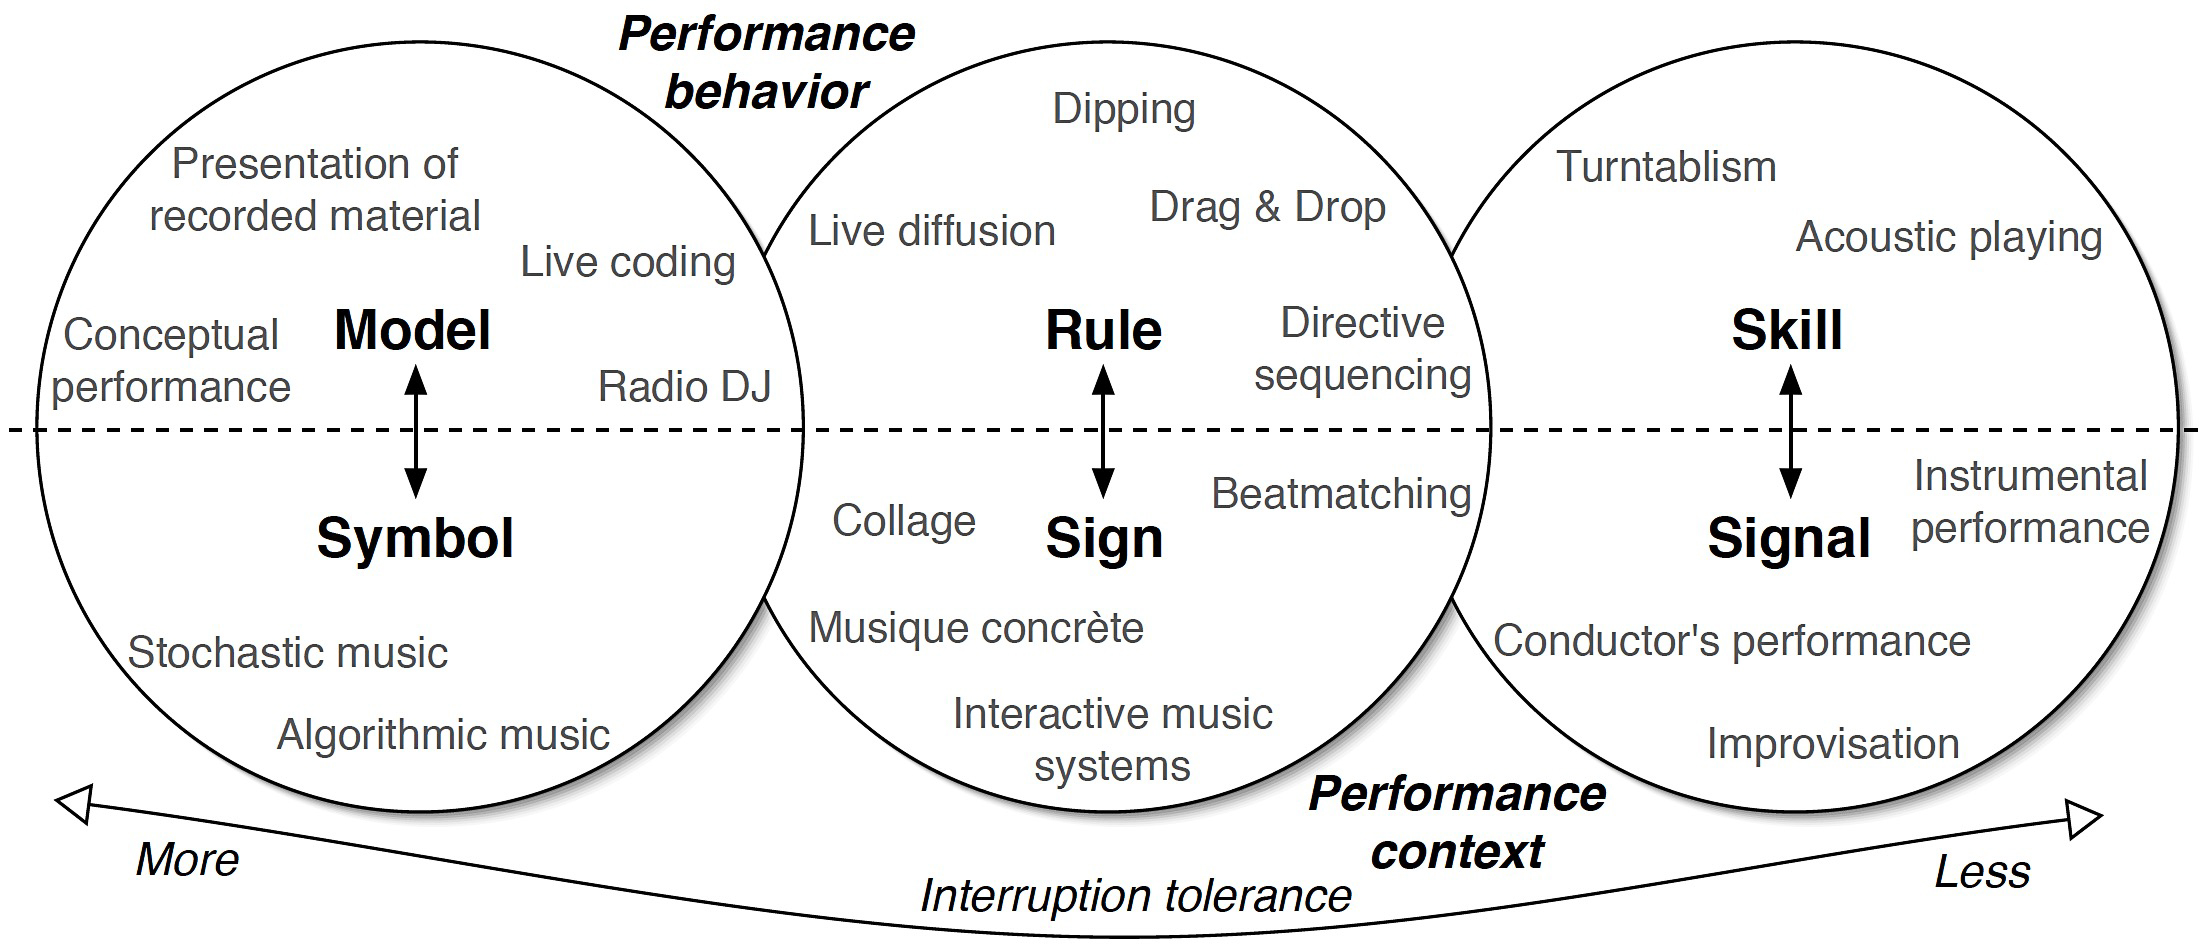
\includegraphics[width=0.83\textwidth]{ch3_malloch_model_of_interaction.jpg}
    \caption[Model of music interaction and performance contexts]{Model of music interaction and performance contexts by \citet{Malloch2006}. Note that \emph{symbol} and \emph{signal} are defined here by the figure's authors and unrelated to the terms as used by \citet{Magnusson2019}.}
    \label{ch3-fig:malloch-model-of-interaction}
\end{figure}

Perhaps the most consequential aspect of the progression from acoustic to electronic, then digital instruments has been the decoupling of the user input from sound production. With any instrument, sound is typically generated and controlled through the various performative actions of its owner. (There are, of course, exceptions to this model, especially in the digital domain, such as instruments that behave autonomously or receive input from arbitrary input data, which are outside of our scope of consideration.) On an acoustic instrument these sound-producing actions, termed \emph{instrumental gestures} by \citet{Cadoz1988}, are physically and mechanically linked to a sonic result, for instance blowing into a saxophone or applying vibrato to a violin string. On the other hand, a digital instrument is not driven by acoustic means and the link between control and sound occurs in the digital realm. Thus, the designer is free to choose any type of input control and any system of mapping controls to sound.

From the designer's perspective this ultimate freedom may be liberating, and is reflected in the increasing quantity, complexity and diversity of new DMIs that have been developed over the last few decades. However this may also present a challenge for designers. Returning to Magnusson's description of the three epistemes, he characterizes the digital era as one in which ``any bodily gesture can be mapped to any sound and there is no natural paradigm at play that we can relate to'' \citep*[p. 34]{Magnusson2019}. While the issue of mapping is a deep area of research and scholarship in its own right (see \citet{os-mapping-2002} and \citet{cmj-mapping-2014} for in-depth reports), here we focus on two more basic inquiries: First, if few technical and conceptual limitations exist, what motivates the design of new DMIs? And second, what methods are effective in the development of novel DMIs that will make them appealing for use in artistic practice?

\subsection{Motivations for designing new instruments}
\label{ch3-sec:motivations-for-designing-new-instruments}

There are a wide range of factors that motivate the design of DMIs, many of which are specific to different end goals. In research settings like NIME, it may be useful to design DMIs that are specific to a particular experimental context \citep{Marquez-borbon2011}. \citet{Morreale2017} survey of DMI designers at NIME found this to be a common approach: out of the 97 instruments included in the study, 38 (39\%) were reported to have been designed as research probes. Depending on various applications and methodological approaches (which may be driven by scientific or artistic goals), these types of instruments may or may not be intended for actual use in musical practice. When considering more widespread audiences for new instruments, social, cultural and economic factors come into play, in particular market and consumer-driven behaviors that influence trends, popularity and visibility of commercial, off-the-shelf instruments \citep{Theberge1997}. The diversity of design approaches (in particular between commercial and research-based designs) was highlighted by \citet{mcpherson2019musical} in a comparison of instruments emerging from different domains including NIME, HCI, and crowdfunding campaigns. 

A study by \citet{Emerson2018} focused specifically on the design of DMIs expressly intended for artistic practice. Out of interviews with ten designers, they identified four primary categories of motivation: facilitating greater embodiment in performance, improving audience experience, developing new sounds, and building responsive systems for improvisation. The study also highlighted different motivations based on the context of participants' practices: those more active in academic settings exhibited more interest new sounds and responsive systems for improvisation, while others who performed in club settings were motivated to improve embodiment and audience experience.

\subsection{DMI design and HCI}
\label{ch3-sec:dmi-design-and-hci}

The diverse motivations for designing new instruments are also reflected in various design approaches and methodologies used. Much of the prevailing discourse on DMI design research comes from the field of HCI, which can provide prescriptive strategies for for all stages of the design process. Early HCI favored systematic approaches, rigid guidelines and formal methods for designing and evaluating human-machine interfaces \citep{Bodker2015}. Examples in DMI research include the formulation of quantitative methodologies like Fitts's Law and Meyer's Law to evaluate target acquisition in the context of musical interactions \citet{Wanderley2002}, and schema developed by \citet{Vertegaal1996c} to match transducers and feedback modes to specific musical functions.

While recognizing the usefulness in these commonly accepted HCI methodologies, Wanderley and Orio also point out the potential limitations to their usefulness in designing music interactions, which are often characterized by idiosyncratic approaches, driven by ``precise artistic demands'' \citep*[p. 67]{Wanderley2002} that yield highly creative and innovative results.

However, HCI has also evolved. While the first wave of HCI was based on models of human information processing theoretically rooted in cognitive psychology, the second wave emerged to include perspectives on technology within social, cultural and organizational contexts \citep{kaptelinin2003}. Rigid and largely quantitative methods gave way to qualitative user-driven and participatory approaches theoretically grounded in situated action, distributed cognition and activity theory \citep{Bodker2006}. The third wave expanded the purview of HCI to accommodate the ubiquitous nature of technology moving beyond the workplace into everyday life and culture, prioritizing experiences, meaning-making and emergent use \citep{Bodker2015}. \citet{Harrison2007} characterize the third paradigm of HCI as phenomenologically situated with a focus on embodied interaction, that can embrace multiple interpretations and yield rich understandings supported by ethnographic and practice-based research approaches.
% \footnote{In this work, our methods are most closely aligned with the second wave, especially in the use of participatory methods, while in the following chapter tends to favor a third wave approach that is grounded in artistic practice.}

\subsubsection{User-centered, human-centered and participatory design}
\label{ch3-sec:user-centered-design}

User-centered design (UCD) is a common approach within HCI where users are systematically involved throughout the design process. \citet{Norman1988} popularized the term, in which the designer should ``ask what the goals and needs of the users are, what tools they need, what kinds of tasks they wish to perform, and what methods they prefer to use'' \citep[as cited in][p. 44]{El-shimy2014}. UCD is less of a method in and of itself than a high level guideline under which several design strategies fall such as those in \citet{greenberg2011sketching}. 

Attitudes towards UCD have evolved over time and, while UCD is still widely used in practice and reference, human-centered design (HCD) has emerged as a subtle but important variation. \citet{Norman2013} describes HCD as a design philosophy and set of procedures that are complementary to more specific areas of focus such as experience design, industrial design and interaction design.\footnote{HCD is also formally defined as an ISO (International Organization for Standardization) standard, however UCD is not.} 
% that add ``deep consideration and study of human needs to the design process, whatever the product or server, whatever the focus'' \citep*[p. 10]{Norman2013}. The \emph{human}-centered scope of HCD provides a the opportunity for wider consideration and different contexts of people in product and interaction design, instead of ``a narrower focus on peoples roles as \emph{users}'' \citep[p. 45]{Steen2011}.
% Human-centered design (HCD) \citep*{Norman2013} has evolved from UCD
% UCD is less of a method in and of itself than a high level guideline under which several design approaches fall. Human-centered design (HCD) is a second term popularized by Norman in \citep*{Norman2013}. 
While similar in both concept and scope to UCD, the \emph{human}-centered scope of HCD allows for a broader consideration of people with regards to design, instead of ``a narrower focus on peoples roles as \emph{users}'' \citep[p. 45]{Steen2011}. This points to a shift that corresponds with trends in HCI: ``Instead of focusing on how specific tools can be designed to help users accomplish specific tasks, the human-centered perspective encourages developers to strive for a better understanding of how people live in the world, and to design systems accordingly'' \citep[p. 45]{El-shimy2014}. 

Participatory design (PD) is an HCD approach that became well-established with second-wave HCI \citep{Bodker2015} and has continued to be relevant in third-wave HCI as well \citep{Muller2012}. It is predicated on the full participation of end-users through all stages of the design process \citep{Steen2011}, and is primarily concerned with the \emph{tacit knowledge} of the involved participants which, according to \citet{Spinuzzi2005}, is hard to formalize and had been missing from early HCI. PD provides several techniques that are relevant to our work here, including ethnographic methods, workshops, low-tech prototyping and mock-up designs \citep{Muller1993a}. However, the roots of PD, which originated in Scandinavia in the 1970s, are also political, and it was envisioned as a way ``to rebalance power and agency among managers and workers'' \citep[p. 1]{Bannon2018}. Some current PD practices have been critiqued as merely UCD by a different name, lacking the original political and activist contexts: 

\begin{quote}
    It is a far cry from earlier work in the field, where Participatory Design not only sought to incorporate users in design, but also to intervene upon situations of conflict through developing more democratic processes. \citep[p. 2]{Bannon2018}. 
\end{quote}

There are instances of PD applied in the design of DMIs. A PD-based methodology was proposed for the design and evaluation of Theremin-based controllers by \citet{Geiger2008}, and PD techniques were applied in the development of audio-haptic interfaces for visually impaired sound engineers and musicians by \citet{Metatla2016}. A participatory approach to music interaction design based on conceptual metaphor theory was also introduced by \citet{wilkie2013towards}. Finally, we note that our own work presented here uses HCD methods that fall under the PD umbrella but without any specific political motivation; therefore we present our approach as HCD and refrain from characterizing it as full PD in deference to the aforementioned objections raised by \citeauthor{Bannon2018}. 

\subsection{Design frameworks}
\label{ch3-sec:design-frameworks}

HCI research has contributed a number of different frameworks for the design and evaluation of new DMIs, While not exhaustive, we highlight a few that help to inform our own specific design approaches. 

A theoretical framework by \citet{Bongers2000a} based on early HCI approaches organized musical interaction as a two way process of \emph{control} and \emph{feedback} described across three categories: \emph{performer-system}, \emph{system-audience} and \emph{performer-system-audience}. This was followed by an explanation of the techniques and technologies (in particular the various sensors to capture different types of performance gestures) necessary to realize the proposed interactions. \citet{Wanderley2004} proposed a design framework for gestural control of sound synthesis comprised of four main elements: \emph{gestures}, \emph{sensors}, \emph{mapping} and \emph{sound production}, which also included \emph{feedback} from the instrument back to the performer. 

Around the same time, Jordà \citep*{Jorda2004, Jorda2004b} introduced several interrelated concepts of musical instruments and practice (\emph{efficiency}, \emph{apprenticeship}, \emph{learning curve}, \emph{diversity}, \emph{freedom} and \emph{control}) towards formulating a conceptual framework that could address diverse needs of different performers appropriately. A separate theoretical framework was subsequently proposed by \citet{Overholt2009} that focused on human-centered design approaches in the combined areas of music performance, HCI and digital technology.

\citeauthor{OModhrain2011a}'s framework for the evaluation of DMIs \citep*{OModhrain2011a} takes a unique approach, prioritizing the various stakeholders involved in the development of a new instrument, including audience, performer/composer, designer, and manufacturer. Another HCI-based evaluation framework is specified by \citet{Young2015a}, emphasizing established, rigorous and flexible techniques to ensure complete and in-depth device appraisals. Finally, \citet{fmorreale:2014} created the Musical Interfaces for User Experience Tracking (MINUET) framework to serve three purposes: reduce design space complexity, specify criteria for design success, and to guide evaluation procedures. The framework divides the design process into two stages. The first establishes design objectives and the second designs the appropriate interaction to meet the established objectives. It establishes a user-centered design approach framed by \emph{people}, \emph{activities}, \emph{contexts} and \emph{technologies} derived from \citet{Benyon2005}, embracing more embodied and participatory methods found in the second and third waves of HCI research.

\subsection{Novel approaches to idea generation and prototyping}
\label{ch3-sec:novel-approaches-to-idea-generation-and-prototyping}

While these frameworks may be helpful in formulating a conceptual design approach, they are generally not oriented towards specific design tools and methods. For our own design work, we wish to develop effective strategies for developing new instruments that will be appealing for musicians to incorporate into their own artistic practice. In particular, we look at two user-driven approaches to generating ideas for new designs: a physical DMI prototyping toolkit and a design workshop methodology. 

\subsubsection{Probatio}
\label{ch3-sec:probatio}

Probatio is a system developed by \citet{Calegario2019} that is comprised of a set of physical modules and accompanying methodology for exploring ideas and developing proof-of-concept DMI prototypes. It is meant to address a few important issues that arise in DMI design: for one, it provides functional constraints to limit the endless possibilities and increased complexity that arises from the separated user input and sound production components of DMIs, which can lead to ``creative paralysis'' \citep{Magnusson2010}. For another, it can help speed up and eliminate bottlenecks for iterative design, facilitating rapid design and evaluation cycles. The Probatio hardware consists of several control blocks, each featuring a different type of input control (ie., buttons, slider, crank, etc.), and different bases and structural supports that can accommodate variable configurations of the control blocks. The hardware is engineered so that the blocks attach magnetically and electrical connections are made automatically. Control signals are then mapped to sound synthesis software, making the prototype instantly playable as soon as one or more blocks are connected. An example Probatio prototype is shown in Figure \ref{ch3-fig:probatio-assembly}.

\begin{figure}[htbp]
    \centering
    \begin{subfigure}[t]{0.485\textwidth}
        \centering
        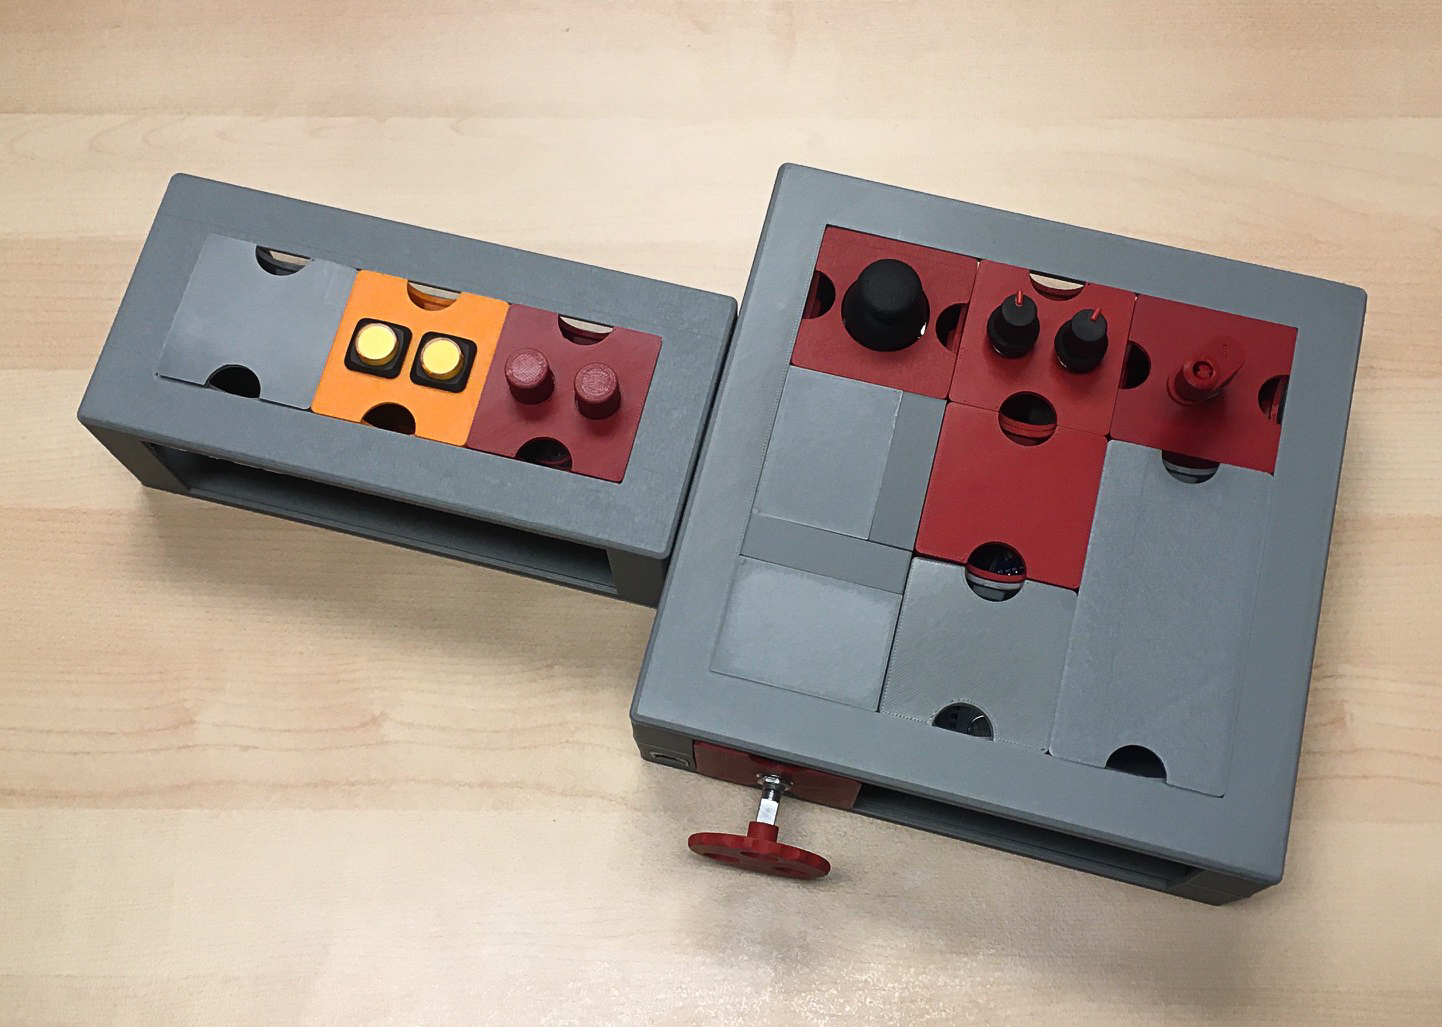
\includegraphics[width=1\textwidth]{ch3_probatio_assembly.jpg}
        \caption[]{A prototype constructed with a Probatio base, structural support and several control modules.}
        \label{ch3-fig:probatio-assembly}
    \end{subfigure}
    ~
    \begin{subfigure}[t]{0.485\textwidth}
        \centering
        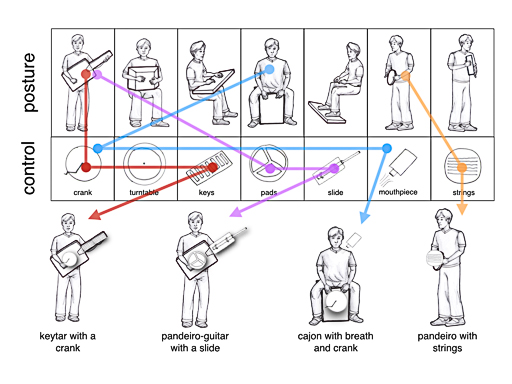
\includegraphics[width=1\textwidth]{ch3_probatio_chart.jpg}
        \caption{Morphological chart suggesting new prototypes by combining features of existing instruments. Drawings by Giordano Cabral.}
        \label{ch3-fig:probatio-chart}
    \end{subfigure}
    \caption[The Probatio toolkit.]{The Probatio toolkit, version 1.0, by \citet{Calegario2020}.}
\end{figure}

The methods that guide the use of the Probatio toolkit are based on Calegario's concept of \emph{instrumental inheritance} in which aspects of existing instruments such as physical structures, playing techniques and specific types of input controls can be explored in different combinations and configurations, yielding entirely new instruments. A morphological chart \citep{Cross2000}, shown in Figure \ref{ch3-fig:probatio-chart}, assists the designer in this process, presenting different postures and controls that can be constructed with the Probatio hardware.

\subsubsection{Magic machines and design fiction}

Another compelling approach to idea generation and prototyping for DMI design comes with ``Magic Machine'' workshops developed by \citet{Andersen2017}. The workshops ``make use of the notion of technology as a `magical unknown' as the starting point for a range of workshop techniques that begin with material exploration'' \citep[p. 4971]{Blythe2016}. In them, participants are prompted to make non-functional low-fi prototypes out of generic crafting materials like cardboard, wood, string, and glue. Once finished, they present their creations, demonstrating their use in imagined scenarios.

The Magic Machine workshops have some basis in design fiction, where concepts and problems can be explored through the development of imaginary scenarios and ``fantasy prototypes'' \citep{Sterling2009}. Importantly, the artefacts that are generated (the non-functional prototypes) are not overly meaningful in and of themselves, and the ultimate aim is not solve any given problem. Rather, the processes of creating and engaging with the ``magical unknown'' serves ``to give temporary body to concerns and questions [and] to consider the potential reality of a world in which such a thing might exist'' \citep[p. 4971]{Blythe2016}.

Andersen has run the workshops is a variety of of contexts for both adults and children, including workshops for the design of new (imagined) musical instruments. The workshop was also utilized by \citet{Lepri2019} in a study that explored diverse values and priorities of different music cultures, backgrounds and contexts.

\subsubsection{Towards design for performance}
\label{towards-design-for-performance}

The Probatio toolkit and Magic Machine workshops present dynamic methods for early ideation stages of DMI design that we are interested in applying to our own work. The workshops offer a creative approach for generating ideas free from technological or practical constraints, while Probatio provides a clearly defined set of tools to construct and test prototypes within an established set of constraints. The next section reports on our own workshop that was styled after the Magic Machines workshop. It includes additional details about Andersen's methods and our own customizations to orient the activities to address our specific goals and inquiries. Later in the discussion (Section \ref{ch3-sec:discussion}) we consider how our own methodology can be complementary to the well-structured Probatio approach to ideation and functional prototyping, and if and where the two can overlap. 

\section{The Design for Performance workshop}
\label{ch3-sec:design-for-performance-workshop}

In this section we introduce the Design for Performance workshop, where expert musicians envisioned and crafted fictional musical instruments. The structure draws from a variety of general methods from UCD and PD that have been mentioned so far: design workshops, non-functional and low-fidelity prototyping, iterative design, and design fiction. The workshop was envisioned as part of a multi-stage design study, with additional phases of the project to follow (See Chapter \ref{ch4-cha} for the workshop results applied in the design of new DMIs, and Section \ref{ch3-sec:limitations-and-future-work} for a discussion on current limitations and future work.)

The workshop structure is based on Andersen's Magic Machine workshops but is revised to direct the outcomes towards the generation of design specifications that could be applied to the development of new performance-ready DMIs. Table \ref{ch3-tab:workshop-activities} provides a side by side comparison of the the Design for Performance and Magic Machine workshop activities (in particular Andersen's musical instrument design workshops \citep*[pp. 30-53]{Andersen2017}) and notes variations between them. In Section \ref{ch3-sec:workshop-activities} we describe each activity in detail.

\begin{table}[thbp]
    \footnotesize
    \begin{center}
        \begin{tabular}{ l c c L{5cm} L{5cm} }
			% % \toprule
\hline
			\hline
            \textbf{Activity} &
            \textbf{DP} &
            \textbf{MM} &
            \textbf{Description} &
            \textbf{Variations} \\
			% % \midrule
\hline
			\hline
            Introduction & X & X 
            & Introduce workshop and set out rules 
            & \\ 
            \hline
            Prompt & X & X 
            & Draw the imagined sound/music you wish to create.
            & MM: The prompt is drawn in permanent marker on hand. DP: Prompt is drawn on index card. \\
            \hline
            Build & X & X 
            & Create non-functional instrument prototypes from provided crafting materials
            & \\
            \hline
            Present & X & X 
            & Each participant presents their instrument with demonstration and explanation.
            & DP: During presentations, the facilitator takes note of defining elements of the instrument and adds them to a whiteboard underneath category headings. \\
            \hline
            Discuss (1) & X & X
            & A short discussion follows each presentation to explore the instrument and its design.
            & DP: Presenter and other participants suggest additional elements to be added to the whiteboard. \\
            \hline
            Evaluate & X &  
            & Participants dot-vote the elements they find most compelling in the design of a new instrument. 
            & DP only. \\
            \hline
            Discuss (2) & X &  
            & A group discussion discussion is held to reflect on voted elements and the prospects for their application in design. 
            & DP only. \\
            \hline
            Document & & X 
            & Each instrument is photographed and documented.
            & MM only. (In DP, photographs are taken during presentations.) \\
			% % \bottomrule
\hline
			\hline
        \end{tabular}
    \end{center}
    \caption[Design for Performance and Magic Machine workshop activities]{Comparison of activities for the Design for Performance (DP) and Magic Machine (MM) workshops, noting any significant differences between the activities.}
    \label{ch3-tab:workshop-activities}
\end{table}

It is important to note that the intended outcomes of the Design for Performance workshops differ from those of the Magic Machine workshops, which are specifically oriented towards building diverse design knowledge and complex understandings ``about technology, rather than of technology'' \citep[p. 1]{Andersen2019}. Our approach seeks to find a middle ground between theoretical knowledge and functional design, connecting the diversity and creative freedom fostered by the Magic Machine activities with a holistic design ecology from ideation to finished product. In this way, the Design for Performance workshop is envisioned as a design tool that can elicit preliminary ideas from a group of expert practitioners and translate them into tangible elements that designers can work with. This may be especially valuable in the DMI design space, where idiosyncratic approaches and highly personalized designs are common, and widespread adoption of new DMIs is limited.

A detailed schedule and script (included in Appendix \ref{axC-sec:schedule-and-script}) was drafted based on Andersen's recommendations to run the workshop at a quick pace and keep a tight timeline. This was found to be an effective strategy to alleviate any potential anxieties or fears of failure that participants could experience during the creative and open-ended design activities \citep{Andersen2017}.

\subsection{Crafting materials}
\label{ch3-sec:crafting-materials}

The main activity of the workshop is for participants to design fictional musical instruments out of provided materials, and the type of materials used can have a large impact on the outcomes of the workshop. 

Through several incarnations of the Magic Machine workshops (that have utilized an array of different crafting materials, from wood and paper to gumdrops) \citet{Andersen2019} provides recommendations and rationales for the selection of materials. Importantly, generic and potentially absurd or impractical qualities of the materials chosen are essential to the activity. In being tasked with building something concrete out of ill-suited materials, the participant is freed from working within practical constraints or following known traditional methods. Furthermore, Andersen emphasizes that any material has the potential to influence the design outcome: particular objects or shapes may suggest typical or obvious uses, which should be avoided. And in the case of musical instrument design, materials may have sound-producing properties that a participant may want to apply in their design. However, Andersen specifies that materials should not be utilized for their acoustic qualities. In this way, the prototypes are explicitly \emph{non-functional} and the design activity is oriented towards the imagining of abstract features and novel forms without concern for feasibility or technical implementation. 

Again, as our goals differed from those of the Magic Machine workshops and we were interested in in tangible design outcomes, we were open to more conventional designs and included some items that might be predictable in their use. For example, each participant was given a large posterboard from which structural shapes could be fashioned, while index cards, colored tape and magic markers would make it easy for participants to draw in graphical user interfaces (GUIs) and other features typical of DMIs.

For the Design for Performance workshop, we selected a wide range of basic items purchased from a dollar store. Materials included:

\begin{multicols}{4}
    \begin{itemize}[noitemsep]
        \item posterboard
        \item index cards
        \item sticky notes
        \item string
        \item wire
        \item rubber bands
        \item popsicle sticks
        \item plastic mesh
        \item paper plates
        \item plastic cups
        \item magic markers
        \item tape
        \item glue
        \item paper clips
        \item scissors
        \item utility knives
    \end{itemize}
\end{multicols}

\subsection{Pilot}
\label{ch3-sec:pilot}

Before the official workshop was held, a pilot test was carried out to run the full workshop from start to finish. Six master's students who were enrolled in a seminar about musical interface design participated. The session was facilitated by the first author with help from an assistant.\footnote{The assistant, Collin Wang, was a master's student supervised by the last author.} The workshop was attended by two colleagues of the facilitator (a music technology Ph.D. student and visiting professor) in order to observe and give feedback. 

The full workshop was run according to the preliminary schedule that had been designed. Afterwards an informal discussion was held with the participants and observers to get feedback and take suggestions for any improvements that could be made. All generally agreed on the activities and format, while details for minor changes were noted and incorporated into the final structure and script.  

While not a focus of this specific study, an interesting contrast between the pilot and official sessions is noted in that the pilot participants were all well-versed in DMI design research. On the other hand, the participants who took part in the official workshops were selected for their experience as active performing musicians and not required to have any preexisting knowledge of DMI design (though some did have some design experience as well). We can envision potentially different outcomes between designers and non-designers. As the pilot study was constructed to test and rehearse the workshop design, and not for data collection and analysis, no further investigation was made around this at the present. However, it suggests a compelling direction to explore for future workshops. 

\subsection{Participant selection}
\label{ch3-sec:participant-criteria-and-selection}

\subsubsection{Research ethics and participant consent}
\label{ch3-sec:research-ethics-and-participant-consent}

Before recruitment began, the Design for Performance workshop was reviewed and approved by the Research Ethics Board Office of McGill University (certificate included in Appendix \ref{axD:reb-ethics-certificates}). This approval requires that studies involving human participants follow specific guidelines for research ethics, to ensure safe handling of data and participants' right to privacy and informed consent. While the participants' names, personal information and gathered data would be anonymized, the proceedings would be photographed and video and audio recorded for later analysis and documentation. Participants would be asked permission to use their likenesses (photos, videos or audio) to be used in public disseminations, including this report. Individuals choosing to opt out would still be welcome to participate fully in the workshop and with their recorded presence removed from any publicized documentation.

\subsubsection{Criteria and recruitment}
\label{ch3-sec:criteria-and-recruitment}

As the workshop was focused on the design of DMIs for use in live performance and intended to be held with expert musicians, we identified three main criteria for prospective participants:

\begin{enumerate}[noitemsep]
    \item They should use, or at least be familiar with, digital, electronic or computer-based instruments for musical performance.
    \item They should maintain an active practice, performing in public on a regular basis (at least five times per year). 
    \item Their performance practice should be related to electronic, electro-acoustic or other musical styles in which DMIs are typically used.
\end{enumerate}

A call for participation was circulated through the following local mailing lists that were likely to reach individuals matching our criteria: 

\begin{itemize}[noitemsep]
    \item McGill University Music Technology Area Graduate Students
    \item Université de Montréal Music Faculty Students
    \item Centre for Interdisciplinary Research in Music Media and Technology (CIRMMT)
    %\footnote{\url{https://www.cirmmt.org}} 
    Members and Students
    \item Eastern Bloc New Media and Production Centre 
    \footnote{\url{https://easternbloc.ca}}
    \item Montréal Contemporary Music Lab\footnote{\url{https://www.labomontreal.com}}
\end{itemize}

Interested parties were invited to complete an online prescreening questionnaire. Recruitment lasted for two weeks and 25 responses were received. Fifteen individuals who met the criteria were invited to participate, divided into two sessions. Five declined or did not respond, leaving a total of ten participants. To accommodate schedules, the workshop was divided into two sessions, with three participants in session A and seven in the session B. Profiles of each participant, including the background information reported on the prescreening, are included with our results in Section \ref{ch3-sec:participant-profiles-and-output}.

\subsection{Workshop activities}
\label{ch3-sec:workshop-activities}

The workshop sessions were held on consecutive days in a large conference room at CIRMMT, a multidisciplinary research center located at McGill University. The first author acted as the facilitator and was assisted by the same master's student who assisted the pilot session. 

Efforts were made to create a comfortable and convivial atmosphere for the participants. The area was spacious and well lit with natural light, and snacks were put out. Tables were arranged together so that participants sat around the outside facing each other. The crafting materials were spread out on a separate table and covered with a cloth when the participants arrived.

\subsubsection{Introduction}
\label{ch3-sec:introduction}

Before starting the workshop activities participants were asked to read and sign an information and consent form that outlined how the workshop would run and explained their rights as participants. Permission was requested for video and audio recording the sessions, as well as for taking photos, to which all participants agreed.

The workshop then formally began, and the facilitator introduced themselves and the assistant, giving additional context and background about the workshop and related research. Then participants went around the room and introduced themselves and gave a short summary of their musical practice, as well as any interest or experience they had in instrument design. Finally, the facilitator presented five guidelines to establish the intended mood for the ensuing activities: 

\begin{enumerate}[noitemsep]
    \item There is no right or wrong.
    \item The activities are short, so move quickly.
    \item Be honest, respectful, and supportive to yourself and the other participants. 
    \item Make sure everybody can be heard. 
    \item Be creative, enjoy the process and have fun with it!
\end{enumerate}

\subsubsection{Activity 1: Prompt}
\label{ch3-sec:activity-1-prompt}

With introductions and administrative affairs concluded, a prompt activity was given. Participants were asked to think of the music that currently make or would like to make, and then instructed to ``draw the music'' on an index card in front of them with a permanent marker. They were given two minutes to complete the activity, after which the workshop moved directly on to the next activity. The given prompt is an adaptation of the Magic Machine version, in which the drawing is done in permanent marker on the participant's own hand. (However in pilot testing, the participants were unanimously opposed to drawing on their hands, so it was moved to an index card instead.)

% Prompts and icebreakers are commonly used in workshop settings to initiate a session, putting the participants at ease and orienting them to the problem at hand. 

Andersen stipulates two important functions that the prompt activity serves: First, it provides the specific context for the workshop focus. In this case, the focus is on designing new musical instruments, therefore drawing the participants' attention to making music in novel and unexpected ways (as suggested by the inherent absurdity of \emph{drawing} music) serves as a primer for the task at hand. Second, the short activity serves as a preliminary task to complete, ``an initial goal\ldots that tests competence and establishes confidence, acting as an on-ramp to an experience'' \citep[p. 5]{Andersen2019}. This eases the transition into to the more substantial design activity that follows, as one creative task has already been completed. Furthermore, any pressures or anxieties that may arise around perceived value or quality in participants' creative outputs are minimized by the short time frame they are given to create their drawings. 

\subsubsection{Activity 2: Crafting non-functional prototypes}
\label{ch3-sec:activity-2-crafting-non-functional-prototypes}

This is the main activity of the workshop, where ``the content of the prompt must be translated into an imagination of the device that produces it'' \citep[p. 5]{Andersen2019}. As discussed in Section \ref{ch3-sec:crafting-materials}, non-functional instrument prototypes are built from rudimentary crafting materials, which moves the focus away from producing high resolution or even technically feasible designs. Instead, the participants are asked to envision and craft a purely fictional instrument that they would want to use, and the materials (and especially their unsuitability for functional instrument design) allow the participant to operate freely and instinctively without concern for implementation or technical constraints.

The following instructions were given to introduce the activity:

\begin{itemize}[noitemsep]
    \item Using the provided materials, you are asked to build an instrument with which you could play the music that you drew.
    \item Bear in mind that you are building \emph{non-functional} prototypes. Your instruments do not need to sound and, specifically, you should not select or utilize materials for their acoustic properties, nor should you be concerned with technical feasibility. 
\end{itemize}

To assist the participants in developing their ideas into tangible designs, we introduced an informal list of eight considerations to refer to while building their instruments. The considerations, listed in Table \ref{ch3-tab:design-considerations} are divided into two categories: \emph{high-level} operational qualities and general characteristics that could describe the instrument's intended use, and \emph{low-level} essential features and fundamental components of the design. While some of the considerations can be classified as functional and non-functional requirements (as defined by requirements engineering \citep{Glinz2007} and commonly employed in systems design), it is important to point out that these elements were empirically chosen based on our own prior knowledge and experience in DMI design, and intended to provide helpful points of reference through the activity. The considerations were presented along with their descriptions before the activity began, then written on a large whiteboard while the participants worked.

\begin{table}[htbp]
    \footnotesize
    \begin{center}
        \begin{tabular}{L{3cm} L{3cm} L{9cm} }
            % \toprule
\hline
            \textbf{Category} & \textbf{Consideration} & \textbf{Description} \\
            % \midrule
\hline
            \multirow{4}{3cm}{Operational qualities and usage} 
            & Functionality 
            & How does the instrument function? 
            \\ 
            \vspace{0.75em}
            & Playability 
            & How do you play it? 
            \\
            \vspace{0.75em}
            & Musicality 
            & What does it sound like, and how does it facilitate musicality? 
            \\
            \vspace{0.75em}
            & Context 
            & Where and how will this be used? (types of venues, solo or in groups, etc.)
            \\ 
            % \midrule
\hline
            \multirow{4}{3cm}{Design features and fundamental components} 
            & Physical form and ergonomics
            & What are the instrument's defining physical characteristics, life size, shape, orientation and posture for the performer?
            \\
            \vspace{0.75em}
            & Interaction methods
            & What kind of controls and user inputs does it have?
            \\
            \vspace{0.75em}
            & Sound production
            & How is the sound produced? (ie., synthesis, sampling, live audio processing)
            \\
            \vspace{0.75em}
            & Feedback
            & What kind(s) of feedback will the instrument provide to the performer?
            \\  
            % \bottomrule
\hline
        \end{tabular}
    \end{center}
    \caption[Design for Performance workshop: Design considerations]{DMI design considerations given for the non-functional prototyping activity.}
    \label{ch3-tab:design-considerations}
\end{table}

The participants were initially given 25 minutes to complete the activity (pictured in Figure \ref{ch3-fig:instrument-building}), though extra time could be allotted if desired. In both sessions, five extra minutes were added, making the total length of the activity 30 minutes. 

\begin{figure}[t]
    \centering
    \begin{subfigure}[]{1\textwidth}
        \centering
        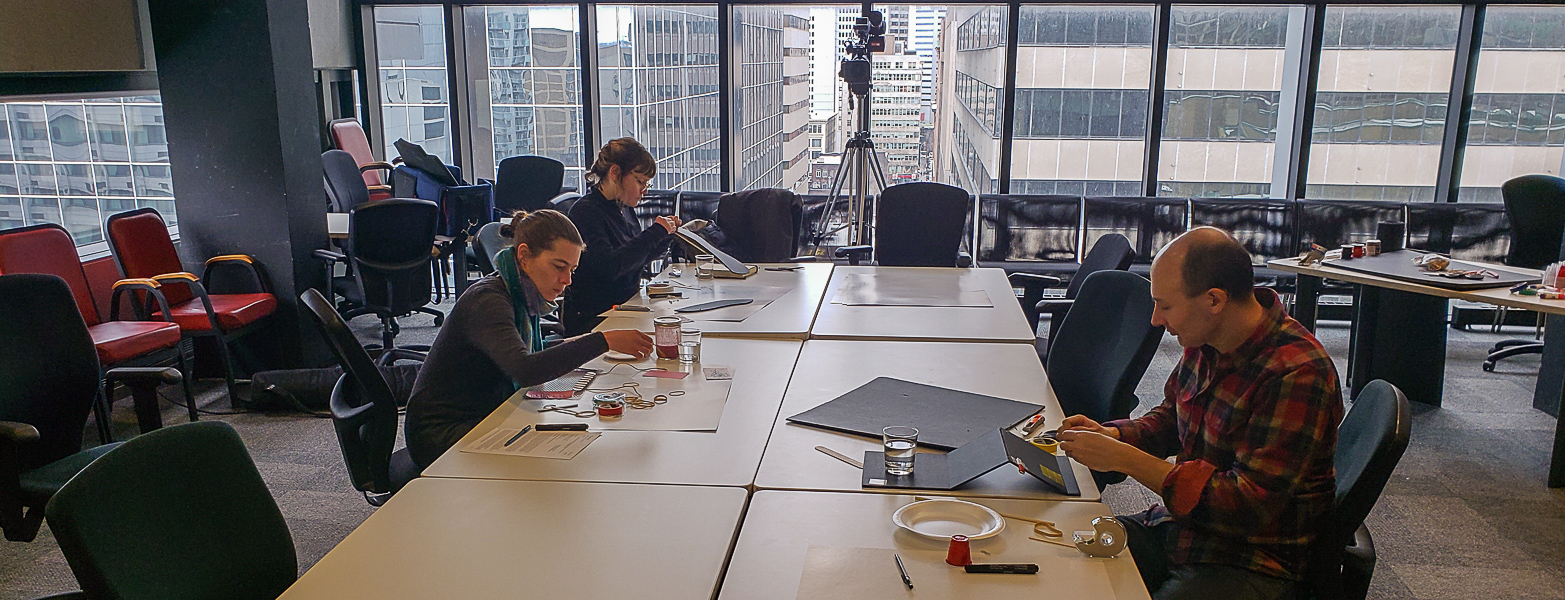
\includegraphics[width=1\textwidth]{ch3_dfp_nfp_A.jpg}
        \caption{Session A.}
        % \label{ch3-fig:keybox-cad}
    \end{subfigure}
    \par\bigskip
    \begin{subfigure}[]{0.59\textwidth}
        \centering
        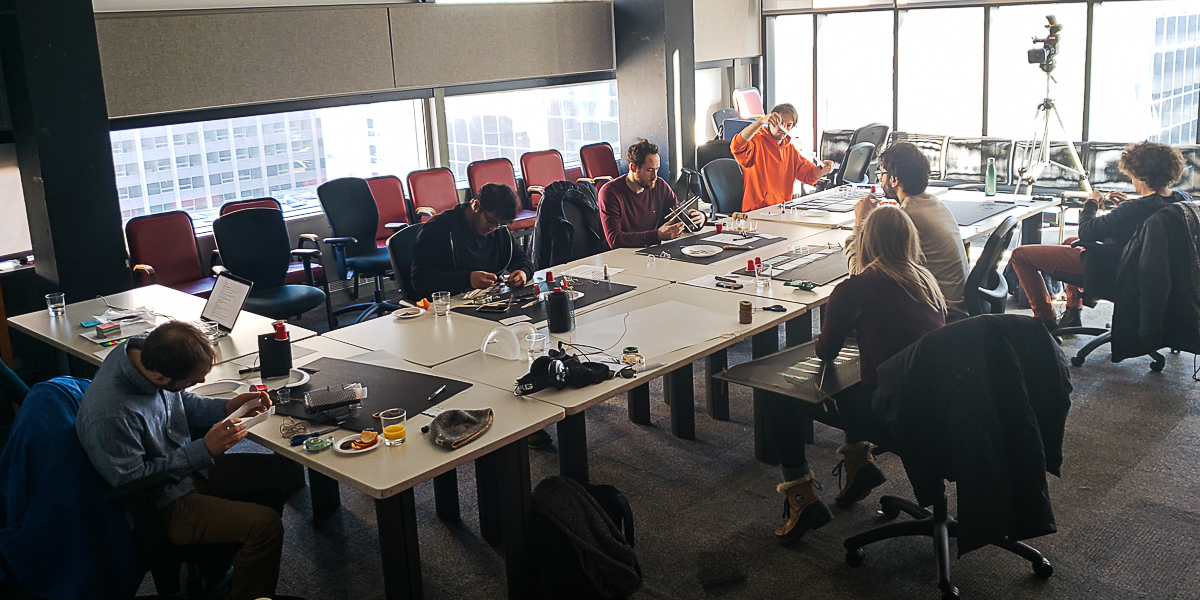
\includegraphics[width=1\textwidth]{ch3_dfp_nfp_B.jpg}
        \caption{Session B.}
        % \label{ch3-fig:stringbox-cad}
    \end{subfigure}
    \begin{subfigure}[]{0.4\textwidth}
        \centering
        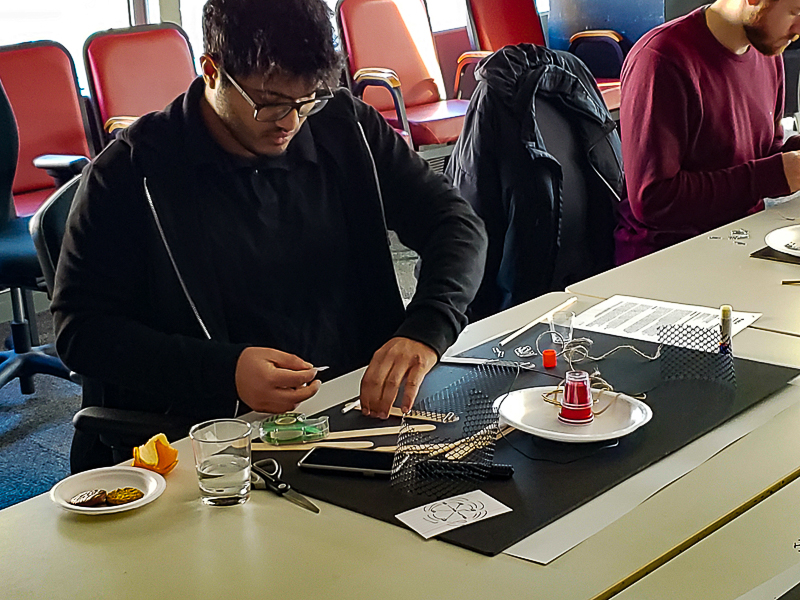
\includegraphics[width=1\textwidth]{ch3_dfp_nfp_B_P4.jpg}
        \caption{Participant P04 in Session B.}
        % \label{ch3-fig:tapbox-cad}
    \end{subfigure}
    \caption[Design for Performance workshop: Activity 2 - Non-functional prototyping]{Participants crafting non-functional instrument prototypes in Activity 2.}
    \label{ch3-fig:instrument-building}
\end{figure}


\subsubsection{Activity 3: Presentations}
\label{ch3-sec:activity-3-presentations}

Next, each participant gave a short presentation and demonstration of their instrument prototype. They began by showing their index card and explaining the music that they had drawn. Then they introduced their instrument, giving a short demonstration of how it was played, and a description of what it was and how it worked. Following suggestions made after the pilot test, the participants were encouraged to explain the links between the ``music'' on their index cards and the instruments, which helped to orient the presentations on the imagined outcomes, rather than the technical details of the fabricated designs. Presentations were allotted five minutes, three for the individuals to present and two for group discussion.

In a departure from the Magic Machine workshop design, an additional element was included during the presentations. While the participants described their instruments, the facilitator listened for ``key elements'' of their designs. Key elements may include essential features, attributes, characteristics that can help to define the instrument. As elements were identified, they were written on sticky notes and posted to the whiteboard, clustered around the eight considerations that had been given in the previous activity. During the presentations and ensuing discussions, the presenter and other participants were encouraged to suggest additional elements which were also added to the board. This method of identifying design elements with sticky notes is common in design research \citep{Fischel2018}. The sticky notes were also color coded by participant to allow us to attribute key elements to individual designs \citep{Reichelt2014}, although ultimately a detailed comparative analysis was beyond the scope of this study.

\subsubsection{Activity 4: Dot-voting}
\label{ch3-sec:activity-4-dot-voting}

The identification of key elements and posting them to the whiteboard was intended to set up a transition in the workshop and allow the group collectively to consider aspects of the designs that would be appealing to incorporate into a fully functional instrument. To facilitate this turn, participants were then asked to dot vote for the elements that they most strongly favored (as shown in Figure \ref{ch3-fig:dot-voting}). 

Dot voting is a common activity in design workshops and collaborative sessions to collaboratively prioritize items from a large set \citep{Gibbons2019} and focus attention for discussion and decision making \citep{Gray2010}. Each participant is given a number of stickers to place by the items of their choosing. When they are finished, the votes are calculated and presented to the group for further action. Various recommendations exist for the appropriate number of votes per participant (\citet{Gray2010} recommends five; \citet{Gibbons2019} recommends 25\% of the overall number or elements to be voted on; another online resource \citep{Lam2019} recommends the formula: $votes=items\div voters\div 2$), which given the number of items and participants in our workshop would equal between 4 and 13 votes per person. Considering these methods and feedback from the pilot workshop, each participant was given 10 votes.

As we will discuss in the presentation of results, the dot voting exercise was less oriented around ranking of essential design elements and more concerned with facilitating a discussion around individual and shared priorities for bringing a new instrument to life. The voting activity was completed quickly and the workshop moved on to a final discussion.

\begin{figure}[htbp]
    \begin{minipage}{0.49\textwidth}
        \centering
        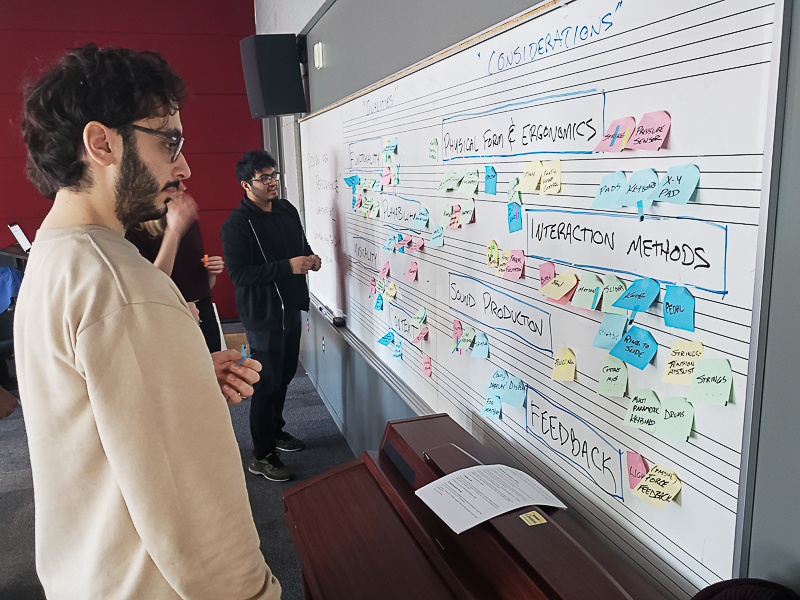
\includegraphics[width=1\textwidth]{ch3_dfp_dot_voting_B.jpg}
        \caption[Design for Performance workshop: Activity 4 - Dot voting]{Session B participants dot voting for essential design elements in Activity 4.}
        \label{ch3-fig:dot-voting}
    \end{minipage}\hfill
    \begin{minipage}{0.49\textwidth}
        \centering
        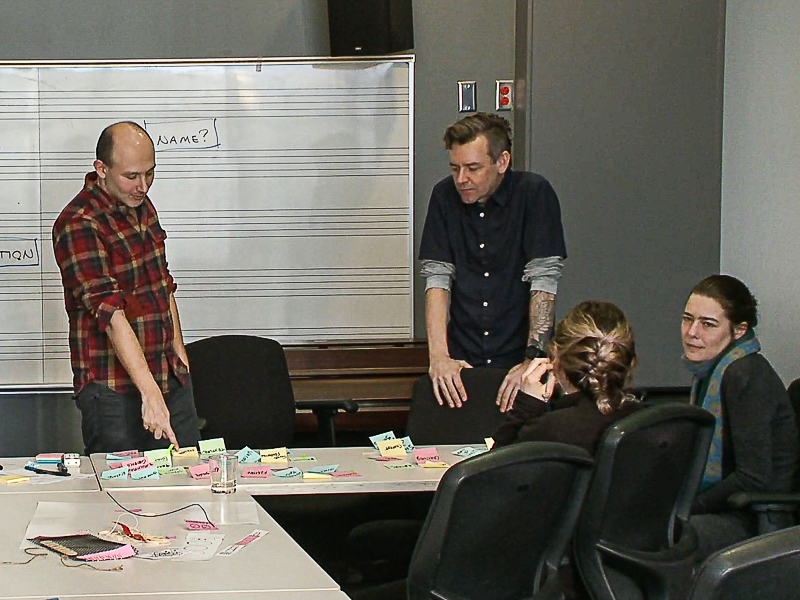
\includegraphics[width=1\textwidth]{ch3_dfp_discussion_A.jpg}
        \caption[Design for Performance workshop: Activity 5 - Discussion]{Session A participants conclude the workshop with a group discussion in Activity 5.}
        \label{ch3-fig:discussion}
    \end{minipage}
\end{figure}

\subsubsection{Activity 5: Group discussion}
\label{ch3-sec:activity-5-group-discussion}

The workshop concluded with an open discussion (shown in Figure \ref{ch3-fig:discussion}) with the facilitator and participants about the identified key elements and prospects for utilizing them and additional aspects of the instrument designs in the development of new DMIs that they would want to use in their own practice. In the discussion, the facilitator also provided information about future steps for the project including the anticipated design of functional instrument prototypes. Ten minutes were allotted for the discussion. The workshop length was planned for 90 minutes, though session B, with seven participants, ran longer and was completed in just under two hours. At the end, the participants were thanked and the workshop concluded.

\section{Results}
\label{ch3-sec:results}

\subsection{Participant profiles and output}
\label{ch3-sec:participant-profiles-and-output}

In addition to the basic background information collected in the prescreening questionnaire, the self introductions at the beginning of the workshop provided additional insights about the participants' own musical and DMI practices. Profiles of the ten participants are shown in Table \ref{ch3-tab:participant-profiles}. 

In their self-introductions, participants were also asked if they had previous experience with designing digital musical instruments, which is included in Table \ref{ch3-tab:participant-outputs}. While this was not a criteria for participation, the participants exhibited varying ranges of personal experience with DMI design. Six of the participants reported at least some previous experience, including P04 and P05 who come from engineering backgrounds and have significant technical knowledge and experience in this area. This is consistent with previous surveys \citep{Magnusson2008, Morreale2017, Morreale2018} that have highlighted the overlap between DMI design and practice (discussed in \ref{ch2-sec:dual-performer-designer-roles}). While not a specific focus for this study, we were interested to see if there were recognizable design trends between performers who were also designers and those who were not. We can also envision a future Design for Performance workshop that investigates the differences between participants explicitly.

\begin{table}[htbp]
    \footnotesize
    \begin{centering}
        \begin{tabular}{ C{0.6cm} C{1.1cm} C{1.3cm} C{1.1cm} C{1.3cm} L{3.2cm} L{4.1cm} }
            
            % \toprule
\hline
            \textbf{ID} &
            \textbf{Years experience} &
            \textbf{Performances / year} &
            \textbf{Use DMIs} &
            \textbf{Design DMIs} &
            \textbf{Instruments played} &
            \textbf{Musical style and description of practice} \\
            % \midrule
\hline
            
            % \multicolumn{6}{|l|}{\rule{0pt}{4ex} \normalsize \textbf{Session A}} \\ \hline
            \multicolumn{6}{l}{ \textbf{Session A}} \\ % \midrule
\hline
            
            P01 &
            14 &
            21-50 &
            Always &
            some &
            synths, radios, DIY instruments &
            experimental improvisation; transmission-based, in situ solo and group performance \\ \hline
            
            P02 &
            23 &
            21-50 &
            Rarely &
            no &
            vocals, guitar, synthesizers &
            rock, noise, drone, free improvisation \\ \hline
            
            P03 &
            30 &
            5-20 &
            Often &
            no &
            guitar, piano, keys, modular synth, misc. electronics, other stringed   instruments &
            Electronic, World music, Experimental, Brazilian; sound and FX for film \\ % \midrule
\hline
            
            % \multicolumn{6}{|l|}{\rule{0pt}{4ex} \normalsize \textbf{Session B}} \\ \hline
            \multicolumn{6}{l}{ \textbf{Session B} } \\ % \midrule
\hline
            
            P04 &
            18 &
            5-20 &
            Often &
            yes &
            piano, guitar, drums, T-stick and Sponge (DMIs) &
            Classical, orchestral, prog rock, metal and blues; more recently into electronic music \\ \hline
            
            P05 &
            20 &
            5-20 &
            Always &
            yes &
            synths, vocals, guitar, DIY instruments &
            Electronic, experimental, pop \\ \hline
            
            P06 &
            13 &
            5-20 &
            Always &
            some &
            sampler, synths &
            Electronic, ambient improvisation; typically plays house parties and dive bars; beat-making (electronic/hip-hop) \\ \hline
            
            P07 &
            10 &
            21-50 &
            Always &
            no &
            guitar, bass, controllers, laptop, Max (software) &
            Contemporary music, noise, electronic; composer \\ \hline
            
            P08 &
            16 &
            5-20 &
            Always &
            some &
            drums, guitar, bass, vocals, piano, laptop, controllers, Ableton Live and Max (software) &
            live electronic music mixed with real instruments: ``Think Radiohead.'' \\ \hline
            
            P09 &
            16 &
            21-50 &
            Often &
            no &
            harp, augmented harp, vocals, laptop, controllers, Ableton Live &
            classical, contemporary, electro-acoustic, free improvisation \\ \hline

            P10 &
            17 &
            5-20 &
            Often &
            yes &
            vocals, guitar, harmonica, Myo (biosignal/motion controller), DIY instruments &
            Ska, folk and electroacoustic; incorporates movement, martial arts and theatre performance \\ \hline
            
        \end{tabular}
        \caption[Design for Performance workshop: Profiles]{Profiles of the workshop participants, from prescreening questionnaire data and self-introductions.}
        \label{ch3-tab:participant-profiles}
    \end{centering}
\end{table}

\begin{table}[htbp]
    \footnotesize
    \begin{centering}
        \begin{tabular}{ c L{5.1cm} L{5.8cm} C{2.5cm} }
            % \toprule
\hline
            \textbf{ID} &
            \textbf{``Draw the music'' description} &
            \textbf{Instrument presentation} &
            \textbf{Instrument classification} \\
            % \midrule
\hline
            
            \multicolumn{4}{l}{\textbf{Session A}} \\ % \midrule
\hline
            
            P01 &
            gestures and organic aspects & 
            modular combination of different sensor inputs that could be mapped and remapped in realtime & 
            alternate instrument \\ \hline
            
            P02 &
            many layers of textures: ``shifting sands of many different sounds [and] melodic lines'' &
            a device for FX processing and cross modulating vocals and guitar &
            instrument-like \\ \hline
            
            P03 &
            layers and textures, slowly going from soft to more powerful &
            a collection of different types of sensors for the performer to interact with sound in many different tactile ways &
            alternate instrument \\ 
            
            % \midrule
\hline
            \multicolumn{4}{l}{\textbf{Session B}} \\
            % \midrule
\hline
            
            P04 &
            audiovisual performance of multicultural music inside a 360° dome representing the world &
            digital/acoustic hybrid acoustic instrument with features of traditional world instruments &
            instrument-inspired \\ \hline
            
            P05 &
            representation of sound propagating through the air, similar to Chiladny plates \citep{Rossing1982} &
            resonant physical structure to excite many different sound processes &
            alternate instrument \\ \hline
            
            P06 &
            circles and orbits, improvising drones and long and short samples shifting over time &
            multifunction workstation: sampler, sequencer, piano keyboard, dual displays &
            instrument-inspired \\ \hline
            
            P07 &
            drops in the water, ripples moving outwards and overlapping &
            stringed instrument held with feet; strings stretched, pulled, plucked, and manipulated &
            alternate instrument \\ \hline
            
            P08 &
            ``any time I hear or feel sound'', music coming from inside body &
            Ondes-Martinot inspired MIDI controller (ring-continuous control) &
            instrument-inspired \\ \hline
            
            P09 &
            harp strings, sound source that is distributed into a living system &
            interface to augment a harp. indirect acquisition of harp sound and manipulation &
            augmented instrument \\ \hline
            
            P10 &
            vertical layers: low basses, middle light and fast, high clear like clouds &
            hyperactive, need to move, two objects tethered to swing around like nunchucks. &
            alternate instrument \\ 
            % \bottomrule
\hline
            
        \end{tabular}
        \caption[Design for Performance workshop: Design outputs]{Design output of the ten workshop participants: description of the ``draw the music'' index cards, their musical instrument prototypes as described in the presentations, instrument classification and previous experience with DMI design.}
        \label{ch3-tab:participant-outputs}
    \end{centering}
\end{table}

% It should be noted that three of the participants are known by the authors. P02 is a PhD researcher who is co-supervised by the last author and has worked with the first author on an unrelated project. P04 was a master's student of music technology at the time of the workshop. While his thesis research was in different area, he had taken a DMI design seminar taught by the second author, with whom he also coauthored a paper on the the redesign of an existing DMI, the Sponge \citep{Tom2019}. Finally, P09 is a harpist whose interest in electroacoustic performance has led to two collaborations with the first author before and after this workshop. These projects are presented in Chapter \ref{ch5-cha}. Given the limited size of the local community involved in DMI practices and its overlap with the research community, we had anticipated that prospective participants might be familiar to us but determined that this should not disqualify them from participation if they met the defining criteria. 

It should be noted that three of the participants are known by the authors. In particular, P09 is a harpist whose interest in electroacoustic performance has led to two collaborations with the first author before and after this workshop. These projects are presented in Chapter \ref{ch5-cha}. Given the limited size of the local community involved in DMI practices and its overlap with the research community, we had anticipated that prospective participants might be familiar to us but determined that this should not disqualify them from participation if they met the defining criteria. 

\subsubsection{Design outputs}
\label{ch3-sec:design-outputs}

Table \ref{ch3-tab:participant-outputs} presents the design output for each participant: their ``draw the music'' index card (as described in the presentations) and the instruments the designed. Figure \ref{ch3-fig:presentations} shows the participants presenting their instruments. Given the abstract nature of the ``draw the music'' task and its express purpose to provide an on-ramp and context for the creative activity to follow, it is unnecessary to discuss the output of the cards themselves and instead focus on the instruments that the participants created. 

\begin{figure}[htbp]
    \centering
    \begin{subfigure}{1\textwidth}
        \centering
        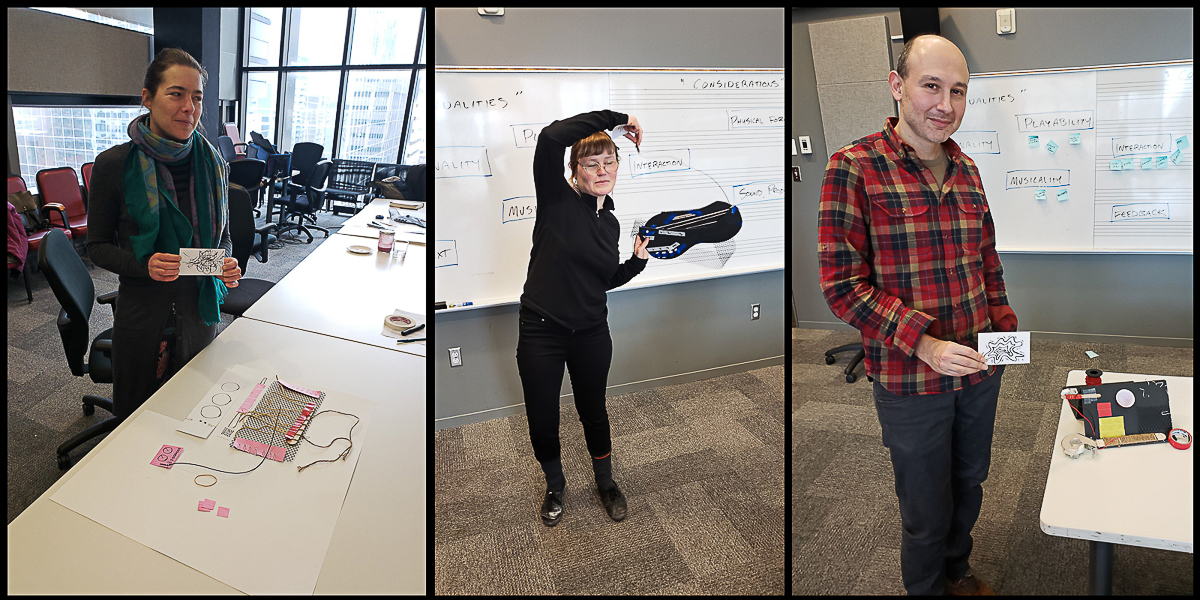
\includegraphics[width=1\textwidth]{ch3_dfp_presentations_A.jpg}
        \caption{Session A: P01--P03 (left to right)}
        \label{ch3-fig:presentations_A}
    \end{subfigure}
    \par\bigskip
    \begin{subfigure}{1\textwidth}
        \centering
        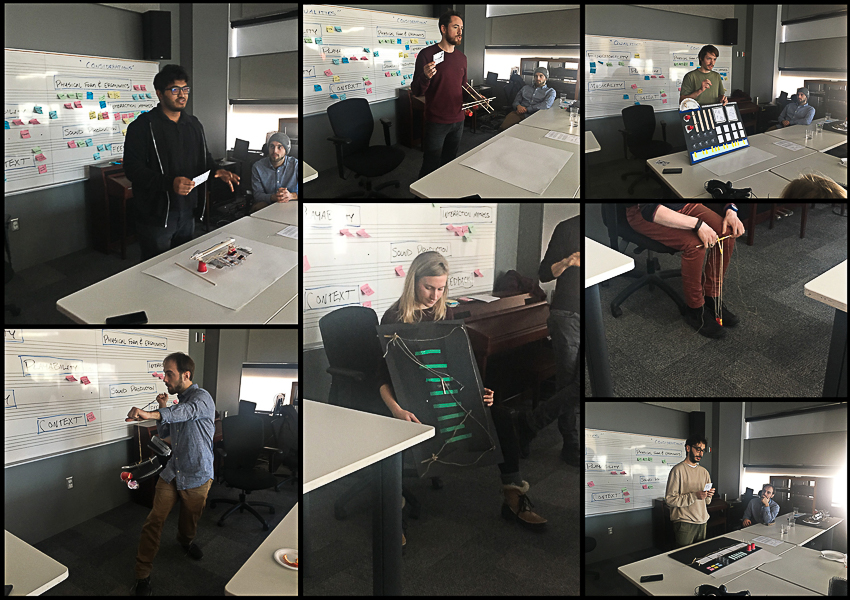
\includegraphics[width=1\textwidth]{ch3_dfp_presentations_B.jpg}
        \caption{Session B: P04--P10 (clockwise from top left)}
        \label{ch3-fig:presentations_B}
    \end{subfigure}
    \caption[Design for Performance workshop: Activity 3 - Presentations]{Participants present their instrument prototypes in Activity 3.}
    \label{ch3-fig:presentations}
\end{figure}

To relate the instruments to existing DMI research, Table \ref{ch3-tab:participant-outputs} also categorizes them according to their similarity to existing instruments, based on \citeauthor{Miranda2006a}'s classification of gestural controllers \citep*{Miranda2006a}:

\begin{itemize}[noitemsep]
    \item \textbf{\emph{Augmented}:} existing instruments extended by the addition of extra sensors which allow the performer to control additional sound and other performance parameters (such as the control of live visuals).
    \item \textbf{\emph{Instrument-like}:} instruments with interfaces modeled closely after existing instruments, but that may be mapped to different functions or sound and musical outputs. 
    \item \textbf{\emph{Instrument-inspired}:} Instruments with interface features that are derived from or inspired by existing instruments, yet are significantly altered from the original.  
    \item \textbf{\emph{Alternate}:} Instruments that are not directly modeled on or necessarily inspired by existing instruments. 
\end{itemize}

Half of the instruments can be classified as alternate instruments. While each was entirely unique, the various forms show the strong influence the materials played on the resulting designs, with each instrument prioritizing physical shapes and textures as the focus of the design. For example, P05 created a resonant physical structure built of many different types of materials (Figure \ref{ch3-fig:presentations_B}, top center). The structure would be excited by touching, tapping, rubbing or plucking different elements, which would generate audio signals to drive multiple different sound processes. 

Four of the remaining five instruments can be identified as either instrument-like or instrument-inspired, taking various elements from existing instruments and repurposing them in different ways. A noticeable trend among this group was to combine the functionalities of several instruments into a single instrument, either to be able to play multiple parts simultaneously like P06's multifunction performance workstation (Figure \ref{ch3-fig:presentations_B}, top right) or to mix them together in creative ways like P02's instrument that would mix and cross-process vocals and guitar (Figure \ref{ch3-fig:presentations_A}, center). 

There was one augmented instrument designed by P09 (Figure \ref{ch3-fig:presentations_B}, bottom center). This participant is an expert instrumentalist with an advanced degree in performance on her instrument, the concert harp. She has been performing electroacoustic music using harp and various external controllers and was clear in her needs and priorities as a performer, which was reflected in the pragmatic approach and practical utility of her design. (As previously mentioned, P09 and the first author are active collaborators whose work is the subject of the following chapter.)

% ...at the time of the workshop P09 and the author the participant and first author had previously collaborated, and would collaborate again, focusing on designing novel technologies for professional performers. 

In Andersen's Magic Machine workshops, the physical objects that are produced are design artefacts. Instead they may serve to evoke inspirations for discussion and conversation within the workshop group, or ``serve as simple vessels for notions and ideas, which are somewhat or completely beyond, what is represented in the model'' \citep[p. 63]{Andersen2017}. This holds true for the Design for Performance workshops as well, and therefore the physical prototypes themselves were not analyzed in depth. Instead the key element identification and dot-voting activities, followed by the post-workshop thematic analysis of the presentations provided a rich understanding of the participants' designs. 

\subsection{Key elements, dot voting, and discussion}
\label{ch3-sec:key-element-identification-and-dot-voting}

In this section, we examine the output of the remaining workshop activities: the key elements compiled during presentations, results and implications of the dot voting activity, and the group discussions that concluded the sessions.

\subsubsection{Key elements}
\label{ch3-subsub-key-elements}

As described in Section \ref{ch3-sec:activity-4-dot-voting}, during the instrument presentations the facilitator, along with the suggestions of the presenter and other participants, identified key elements of the instrument designs and posted them on a whiteboard. We intentionally refrained from giving a strict definition for what constitutes a ``key element'' in hopes of drawing out intangible aspects of the designs in addition to more obvious and concrete elements. Given the short format of the presentations (three minutes to present and two minutes for discussion), this was not an exhaustive list, however with the active participation of the whole group we attempted to capture most of the essential elements of each instrument. The full list is included in Appendix \ref{axC-sec:key-elements-and-dot-voting-results} showing the elements corresponding to each participant's instrument, as identified from the color-coded sticky notes.  

36 elements were recorded for the three instruments in Session A and 70 elements identified for the seven instruments in Session B, for a total of 106 (averaging 10.6 elements per instrument). As the elements were posted during the presentations, they were clustered around the eight considerations the participants had been given at the start of instrument prototyping exercise (see Table \ref{ch3-tab:design-considerations}). These weren't intended to be strict categorizations and the classification of some elements was ambiguous, but this provided a basic structure that helped to reveal where the attention of the designs was focused. Figure \ref{ch3-fig:key-elements-by-category} shows the distribution of elements across the categories. 

\begin{figure}[htbp]
    \centering
    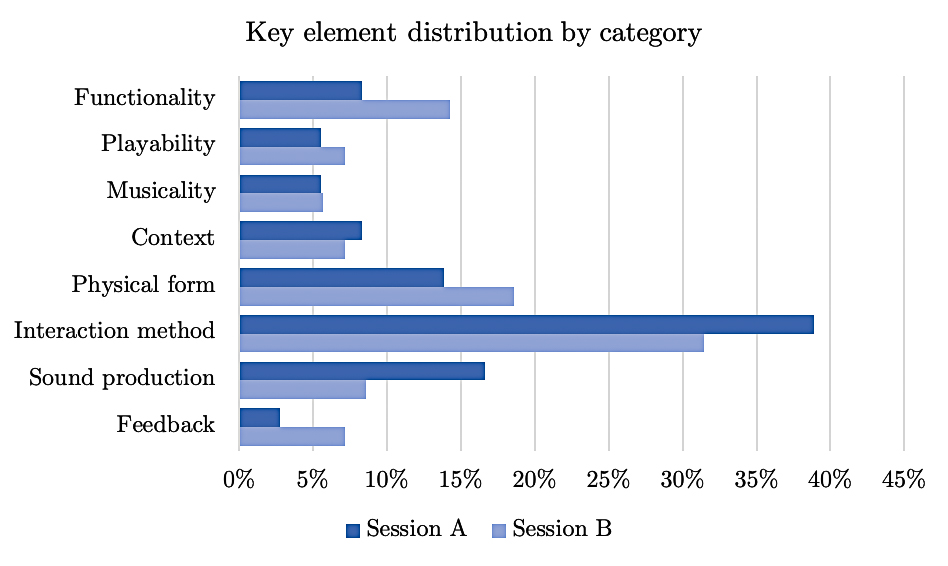
\includegraphics[width=0.75\textwidth]{ch3_key_element_categories}
    \caption[Design for Performance workshop: Key elements by category]{Distribution of key elements by category (design considerations), shown as percentages of total elements identified. For Session A, \emph{N}=36; for Session B, \emph{N}=70.}
    \label{ch3-fig:key-elements-by-category}
\end{figure}

The most common category was \emph{interaction methods}, with roughly one third of all elements related to how the performer would interact with the instrument, naming specific types of controls (like knobs or keys) or describing techniques for playing the instrument (touching, bowing, moving, etc.). While both controls and playing techniques were classified into one category here, it is worthwhile to note that they are not strictly orthogonal. A DMI design study by \citep{Marshall2009b} had found that musicians tended to use the same control with different interaction techniques and playing strategies. Nonetheless, the frequent mention of both physical controls and instrumental technique highlights the embodied connection between a performer and their instrument that has been a strong theme in DMI research \citep{Emerson2018,Magnusson2007} and third wave HCI \citep{Harrison2007}). On the other hand, the prevalence of this category may also be due in part to the structure and pace of the presentations, where describing these elements (along with physical form, which was the second most frequent category) gave the most succinct description of an instrument in a short time. 

Another insight from the categorizations is that overall, the more abstract ``operational qualities and usage'' considerations of \emph{functionality}, \emph{playability}, \emph{musicality}, and \emph{context} received far less attention than the more concrete ``design features and fundamental components'' of \emph{physical form}, \emph{interaction methods} and \emph{sound production} (though the fourth category \emph{feedback} was the least identified of all). Again, we refrain from reading too much into this, because the more objective elements may have simply provided the quickest and most direct way to describe the instruments.

\subsubsection{Dot voting and group discussion}
\label{ch3-sec:dot-voting-and-group-discussion}

Following the presentations, the participants dot voted for the elements that they would most want to be incorporated into a new instrument design. Table \ref{ch3-tab:dot-voting} shows the top dot voted elements from each session and Appendix \ref{axC-sec:key-elements-and-dot-voting-results} shows the votes for all elements.  

\begin{table}[htbp]
    \footnotesize
    \begin{centering}
        \begin{tabular}{lc|lc}
            \multicolumn{2}{c}{\textbf{Session A}} &
            \multicolumn{2}{c}{\textbf{Session B}} \\
            % \toprule
\hline
            \textbf{Element} & \textbf{votes} &
            \textbf{Element} & \textbf{votes} \\
            % \midrule
\hline
            playful unreliability & 3 & synthesis & 5 \\
            textures & 3 & audiovisual experience & 4 \\
            modular & 3 & pressure sensor & 4 \\
            organic & 2 & plucking & 4 \\
            move while you play & 2 & MIDI output & 3 \\
            blending & 2 & portability & 3 \\
            radio & 2 & strings & 3 \\
            touching & 2 & & \\
            % \bottomrule
\hline
        \end{tabular}
        \caption[Design for Performance workshop: Dot voting results]{Prioritized key elements as ranked by the dot voting activity. In Session A, elements receiving more than 1 vote are shown, and in Session B, elements receiving more than two votes are shown.}
        \label{ch3-tab:dot-voting}
    \end{centering}
\end{table}

In planning the workshop, we imagined the key element identification and dot voting steps could serve two possible functions. First, it could indicate areas of consensus (or disagreement) between the participants' designs that could inform the discussion around prospects of employing elements into functional instruments. Second, we hoped that the process on its own might suggest clear directions to orient our future functional designs. 

In Session A the closing discussion followed the dot voting with conversations around several of the prioritized elements. There was a high amount of agreement despite the individual instruments being very different. In particular, the participants valued modular instrument designs that could facilitate mixing and rerouting of signals, and allow the instruments to be flexible for use in a variety of ways. 

Additionally, the quality of \emph{playful unreliability} was popular, where an instrument might behave in non-deterministic or unexpected ways, leading to novel sounds and new ways of performing. This seemingly runs counter to one of the findings of \citeauthor{Magnusson2007}'s survey (discussed in Chapter \ref{ch2-cha}, Section \ref{ch2-sec:dual-performer-designer-roles}), in which many respondents were intolerant of this quality in digital instruments. However the underlying assumptions aren't necessarily the same. The viewpoints of our workshop participants, who are active in improvisation and experimental performance, are consistent with Chadabe's \citep*{Chadabe1984} description of \emph{interactive composing}, in which the performer ``shares control of the music with the information that is automatically generated by the computer, and that information contains unpredictable elements to which the performer reacts while performing'' \citep[p. 23]{Chadabe1984}. Thus the difference lies in the performer's understanding and expectation of an instrument. If the unreliability is intentional, it can be coopted into their performance; if unintentional, it is more likely viewed as a flawed or malfunctioning instrument. 

In Session B, the discussion was relatively short as the session was nearing the two-hour mark and there was a sense that the participants were ready to leave. In addition, as there were so many elements on the board and a wide variety of elements receiving votes, it was difficult to facilitate a conversation around the distinct elements or specific design ideas. However, a comment by P07 provided a valuable observation:  

\begin{quote}
   \emph{ I'd say that you can sum [an instrument] up with keywords, but sometimes what makes it special or good are all the keywords together. If you take some of the words that were thought by different brains [and put them together in a single instrument], it can turn out like Frankenstein.}
\end{quote}

\section{Thematic analysis}
\label{ch3-sec:thematic-analysis}

The preceding quote elucidates the challenge of moving from the individual and idiosyncratic ideas of the participants (as expert performers and end users), to tangible design specifications that can drive instrument designs. Our intent was for the sessions to serve as a space to freely generate ideas which, as seen in the creativity of the designs, was successful. However a systematic understanding of the participants' designs failed to materialize. We can suggest two reasons for this. First, the real time identification of key design elements during the fast-paced presentations may not have captured the full essence of the instruments, especially more nuanced or less pronounced elements, and (as reflected in P07's comment) the connections between them. Second, though not explicitly intended in the workshop design, the ensuing activities (key element identification, voting and discussions) were largely organized in a top down manner, structured around the the eight pre-defined considerations given during the workshop activity. 

To better understand the workshop results, an exploratory thematic analysis was conducted using the methodology presented by \citet{Braun2006}, which we had previously employed for the qualitative analysis of an online survey (see Section \ref{ch2-sec:results}). The goals of the thematic analysis are to organize and describe a data set in rich detail, and the methods are flexible to accommodate a variety of approaches. We chose an inductive approach, similar to the constant comparison method found in grounded theory \citep{Strauss1994}, in which the data set is coded from the bottom up, and avoids fitting it to any preexisting framework.

Our analysis included the following steps: 

\begin{enumerate}[noitemsep]
    \item Presentations of the ten participants were transcribed from the video recordings. 
    \item A round of open coding was performed on the transcribed presentations, where all codeable incidents were identified and assigned preliminary codes. 
    \item In a second round of coding the incidents were compared to one another to identify similarities and relationships between them, yielding the final set of codes. 
    \item The codes were then sorted into themes, which were in turn reviewed and refined, then defined and named. 
\end{enumerate}

The initial round of open coding was performed using Microsoft Excel, while the rest of the analysis was completed with NVivo\footnote{\url{https://www.qsrinternational.com/nvivo-qualitative-data-analysis-software/}}, qualitative data analysis software. NVivo contains a powerful set of features that are particularly useful to develop a rich understanding and and deep insights out of qualitative data, such as the ability to synchronize video and audio files to text transcripts, and to link the data set to different \emph{nodes} (emerging codes and themes) in a searchable database. This underlying structure made it possible to explore the data from different perspectives throughout the process, which helped us determine our complete list of codes and themes. 

In all, 152 incidents were coded across the ten presentations, yielding 56 individual codes categorized across eleven themes. The full list of codes and themes, along with their mentions by participant, is included in Appendix \ref{axC-sec:workshop-presentations-thematic-analysis-full-results}. 

\subsection{Design specifications}
\label{ch3-sec:design-specifications}

To move from open exploration in the workshops to tangible design implementations, we examined the six most common themes (which were mentioned by at least half of the participants) and formulated five of them into a set of design specifications. In Table \ref{ch3-tab:themes-and-specs}, we list each theme with its description, a representative participant quote, and resulting design specification. 

\begin{table}[htbp]
    \footnotesize
    \centering
    \begin{tabular}{L{0.38\textwidth} L{0.28\textwidth} L{0.26\textwidth}}
        % \toprule
\hline
        \textbf{Description} &
        \textbf{Quote} &
        \textbf{Specification} \\
        % \midrule
\hline
        \multicolumn{3}{l}{\textbf{\emph{Interaction styles and input control}}} \\
        Embodied physicality; materials, shapes and textures for unique tactile interactions; strings, movement and position sensing, as well as standard input controls. & 
        ``I bring in different types of textures that you can touch. Touching is an important part of it.'' (P03) & 
        Combine conventional and novel interface elements that prioritize embodied, physical, and material-oriented interactions. \\
        % \midrule
\hline
        
        \multicolumn{3}{l}{\textbf{\emph{Signals, connections, and mapping}}} \\
        Flexible, user-definable signal routing and input mapping; Eurorack-style patching, touchscreen and hardware signal matrixes, configurable wireless networks. &
        ``There could be some kind of tactile matrix that you could change to get different sensors.'' (P01) &
        The instrument should feature flexible audio and control signal routing and mappings. \\
        % \midrule
\hline
        
        \multicolumn{3}{l}{\textbf{\emph{Sound production and processing}}} \\
        Sampling, mixing, and layering sounds; processing external audio; synthesizing and modulating audio signals; exciting resonant acoustic objects for signal generation. &
        ``The idea is to get a physical structure that is resonant by itself \ldots then just one stroke, one gate, propagates one signal all over the other instruments.'' (P05) &
        Generate sound via external audio input and resonant acoustic features; sample, synthesize, mix, modulate and process audio signals. \\
        % \midrule
\hline
        
        \multicolumn{3}{l}{\textbf{\emph{Extending (or inspired by) existing instruments}}} \\
        Referencing specific features, functions and playing styles of other instruments. &
        ``This is like the poor man's version of [the Ondes Martinot], in that the original instrument is really impractical and it's really weird and old technology.'' (P08) &
        Mix familiar elements of existing instruments with novel methods of interaction and sound production. \\
        % \midrule
\hline
        
        \multicolumn{3}{l}{\textbf{\emph{Versatility}}} \\
        Versatile, multipurpose instruments that can be used in different ways and contexts; multifunction controls and interchangeable modules. &
        "I wanted something that makes singing, while playing guitar, while doing lots of stuff to your voice, plus your guitar, easier." (P02) &
        The instrument should feature multiple modes or modules of operation that allow for a variety of playing styles. \\
        % \midrule
\hline
        
        \multicolumn{3}{l}{\textbf{\emph{Performance environment}}} \\
        Large-scale performance environments, audiovisual elements, video projections, immersive spaces and audience interaction. &
        ``So I am imagining I'm playing in a dome-like structure, with the world map projected on to it.'' (P04) &
        \emph{none} \\
        % \bottomrule
\hline
        
    \end{tabular}
    \caption[Design for Performance workshop: Themes, quotes and specifications]{Six themes generated from the workshop analysis with description, exemplar quote and resulting design specification.}
    \label{ch3-tab:themes-and-specs}
\end{table}

No design specification was formulated for the \emph{performance environment} theme. As we will discuss the following section, the specifications would be applied to the design of instruments using an existing instrument framework, which carries its own set of constraints especially in terms of size, available materials and fabrication methods. While the design of large-scale audiovisual environments was appealing to several workshop participants and offers possibilities for future designs, it is beyond the practical scope of our current project. 

\section{Discussion}
\label{ch3-sec:discussion}

The Design for Performance workshops were developed as a strategy to generate novel ideas for new DMIs, using methods from contemporary HCI and participatory design, which prioritize qualitative and situated approaches to design and evaluation. By bringing in expert musicians, we aimed to leverage their tacit knowledge and experience of real-world performance practice in hopes that their input could direct the design of instruments that would be appealing and viable to be taken up into musical practice. The choice to use of design fiction as a primary methodology was made for two reasons. First, by removing technological constraints and considerations, the participants were allowed to freely build non-functional prototypes with a focus on their musical practice, without worrying about the feasibility of implementing their designs into functional instruments. Second, the activity, as well as the ``draw the music'' prompt before it, situated the participants and designs in a fictional narrative of their own imagining. The playful aspect of the activities - the inherent absurdity of drawing music, and the ``arts and crafts'' approach to building an instrument - urged the participants to be creative and unconventional in their endeavors. 

From a designer's point of view, this approach to capturing ideas generated by musicians, especially those that are highly creative and not bounded by the limitations of technical feasibility, can help to stave off potential creative paralysis, bringing in fresh ideas and a better understanding of priorities for performance.

\subsection{Tools for design}
\label{ch3-sec:tools-for-design}

A large part of the methodology designed for this project was adopted from Andersen's Magic Machine workshop playbook. Regarding the prospects for these methods to be used by other researchers, \citeauthor{Andersen2019} proposes that ``the multiplicity of highly personal and interpretive content might serve as an additional and complementary resource to design and HCI workshops, which can then in turn be analyzed, annotated or simply challenge designers'' \citep*[p. 12]{Andersen2019}. Our work here aims to apply the unique and imaginative approach of of design fiction to collaborate with expert musicians to generate creative new ideas and elements for the design of new instruments. 

HCI has informed several well-structured approaches to DMI design, which were reviewed in Section \ref{ch3-sec:background}. With the Design for Performance workshops we aim to align our methods with current and emerging HCI concerns, especially focusing on embodied interaction, phenomenology and qualitative methods of analysis. We find this approach to be complementary to trends in musical interface design which may combine formal engineering and technical know-how with creative practice, and where the lines between functional design and musical composition may become blurred. 

The path from idea generation to the creation of functional playable instruments is similar to \citeauthor{Calegario2019}'s Probatio \citep*{Calegario2019}, in which an entire design cycle is formed. For Probatio this is achieved in a rapid succession, often in a single workshop session where ideas can be generated and directly explored in hardware, which allows for instant testing and evaluation, and rapid iteration. For this project, we envision the similar progression, but occurring on a longer time frame (including the Design for Performance workshop and subsequent iterative instrument designs), and generating high fidelity prototypes that ultimately can be suitable for use in artistic practice. 

The Design for Performance workshop is intended to be one element of a larger design ecosystem. We envision an iterative design sequence in which multiple workshops can be held to evaluate and refine the resulting instrument designs, similar to the method employed by \citet{Absar2015}, where a sequence of three panels iterated on the development of auditory feedback to assist navigation of a visual information system. An iterative process like this could also employ the Probatio toolkit as a step in the design cycle: Ideas generated from the non-functional prototype designs could be explored in low-fidelity functional models with the Probatio hardware before moving towards the design of high-fidelity prototypes that would be viable for real world use.

\subsection{Limitations and future work}
\label{ch3-sec:limitations-and-future-work}

\subsubsection{COVID-19 and the ongoing suspension of in-person research }

In our own work we have applied the design specifications that were drawn from the workshop to the development of three new DMIs, which are intended to embody several of the aspects that emerged from the workshop participants' designs (which is the subject of the following Chapter). Future workshops were planned to present the prototypes back to the participants for evaluation and feedback. Unfortunately, at the time of writing they have been indefinitely postponed as the COVID-19 pandemic has forced the temporary closure of university research laboratories and suspension of in-person research until the health risks are alleviated. 

While COVID-19 represents a serious and ongoing situation around the world, we remain optimistic that it will be brought under control in due time. As such, while it is disruptive to our immediate applied research plans, we look forward to continuing our design research in-person with participants when it is safe. Additionally, while we haven't applied it this particular situation, there are a variety of tools and methods available to conduct DMI workshops and evaluations remotely through videoconferencing and asynchronous activities (such as recording and uploading practice sessions). However, this requires a thorough evaluation of potential methods and ramifications of this approach, and is not planned for this particular project. 

% \subsubsection{General vs. individual users}
\subsubsection{Generic vs. idiosyncratic design}
\label{ch3-sec:generic-vs-idiosyncratic-design}

The comment by P07 in the closing workshop discussion brings to mind the idea of specificity in design. The participants each created an instrument that was personalized for their own needs and practice, and by combining elements of several different instruments into a single design (the Frankenstein instrument), the essence of any single one may be lost. 

On one hand, we are motivated to orient our designs to address areas of concern for general performers. This is shown through our analysis of the workshop designs and presentations, which found many design elements that were shared by several of the participants. This presents the opportunity to design instruments that could be used by different performers across different contexts, possibly improving an instrument's chance for long-term and widespread adoption. On the other hand, P07's comment speaks to the idiosyncrasy that characterizes field of DMI design, especially where design and performance roles commonly overlap. 

While this issue is not covered in depth here, our continued work explores both angles, first through the design of multiple DMIs intended for a nonspecific user and encapsulating several elements of the participants' designs (Chapter \ref{ch4-cha}), and then though a focused collaboration with a single performer to develop bespoke interfaces for their unique musical practice \ref{ch5-cha}. 

\subsection{Conclusion}
\label{ch3-sec:conclusion}

Here we have reported on a novel approach to generate ideas for the design of new DMIs based on a design workshop methodology that employs design fiction, allowing workshop participants to freely imagine and craft non-functional instrument prototypes. The workshop design is adapted from Andersen's Magic Machine Workshops ~\citep{Andersen2017} and is informed by theories for DMI development based on previous design frameworks and HCI literature. In particular the approach emphasizes the tacit knowledge of the participants, in our case, expert musicians, towards the development of new instruments that would be appealing for performers to take up into real-world use. 

We began by reviewing previous research around DMI design, including motivations for the design and use of new instruments, and various design frameworks that have been proposed. Then we introduced the Design for Performance workshop, which we ran with 10 participants divided into two sessions. We have presented the methodology and results, which included thematic analysis of videorecorded participant presentations and discussions. We found that several design aspects were shared across many of the participants' designs, which we used to develop a list of design specifications. 

As a continuation to this project (which is presented in Chapter \ref{ch4-cha}), we have applied these specifications to the design of three new instruments that are intended to embody many of the desirable aspects presented by the workshop participants. We also envision future workshops, not only to design new instruments, but also to present our current and ongoing designs for feedback and continued iteration. 

Beyond the generation of practical design specifications based on the outcome the workshop that we ran, we also present this research as a methodological contribution of a unique and creative approach to early design stages of idea generation and non-functional prototyping that can serve as the initial steps towards the development of high quality, functional and finished prototypes. These methods, while developed for DMI design, are appropriate for a wide range of applications with within and beyond the creative arts. 


%%%%%%%%%% END OF MAIN TEXT %%%%%%%%%%%%%%%%%


Introductory body text comes here. 
Just replace the text of the template with the text for your article.
Introductory text does not normally have a printed section heading, the default heading "begin article" in double angle brackets is an instruction for the typesetter and should be left as it stands.
Exception: only if the introductory remarks contain subsections (with level-B headings), then the entire introductory section gets a level-A heading, typically ``Introduction'' or perhaps something more exciting.

Starting each sentence on a new line in the LaTeX source can be helpful for the editors in preparing an article for submission to MIT Press.

Use of additional packages, beyond what are included in this template and the cmjStyle.sty (and cmjStyle-pdftex.sty) documents should not be necessary and is discouraged. 

For style questions not answered here, visit http://mitpress.mit.edu/cmj to see the submission guidelines and previously published articles.  
Most issues include a freely downloadable feature article.  
Questions may be directed to cmj-editor@mit.edu; please put [CMJ MS] in the subject line.

\parskip 18pt

%------------------------------------------------
%
% format for Heading-A style
\section{Format for Heading-A Style}

Insert body text here.  
Use the Heading-A style for headings of major sections.
Note that CMJ does not use section numbers for any level of heading.

\vspace*{24pt}

% format for Heading-B style
\subsection{Format for Heading-B Style}

Insert body text here.  
Use the Heading-B style for headings of subsections.

% format for Heading-C style
\subsubsection{Format for Heading-C Style}

Insert body text here.
Use the Heading-C style for headings of sub-subsections.

In the initial manuscript submission, you are encouraged to include figures (with captions) inline with the text, for ease of reading during the review process. 
All figures will need to be grayscale (i.e.,~monochrome) and sufficiently high-resolution for print (300 dpi), at the latest by your final submission.
Figures must be referenced in the text, either directly in the text or as a parenthetic aside, e.g.~``(see Figure~\ref{fig:myFigure}).''
Do not reference figures with terms of relative location like ``above'' or ``below,'' however.
When an article is typeset, figures are never embedded in the text and you do not know exactly where the image will appear in relation to your text.
For the review process, simply place the LaTeX figure definition immediately after the first paragraph referring to the image.

% include figures in text with captions for initial submission, like this:
\begin{figure}[]
\begin{center}
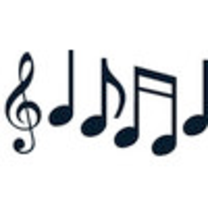
\includegraphics{myFigure}
	% No need for file extensions here! 
	% This is useful at final submission, when MIT Press and LaTeX need different image formats for the same image
	% This template is already set up to look for image files in the Figures subdirectory, so that's where to put your image files. 
\caption{Insert Figure caption here.}
\label{fig:myFigure}
\end{center}
\end{figure}

Tables must also be cited in the text, as with Table~\ref{tab:myTable}. Tables in \emph{CMJ} do not have ``captions'' as such. A table has a title, which should be concise. If absolutely necessary for understanding the table, additional information can be included in a footer, although that is not required. When typeset, tables will not have vertical rules.

% include tables in text with captions for initial submission, like this:
\begin{table}[]
\caption{Sample Table with a Title}
\centering
\begin{tabular}{lccr}
  \hline
  \textbf{Column} & \textbf{Headers} & \textbf{Might Look} & \textbf{Like This}  \\
  \hline
  one & 2 & 3 & IV \\
  five & 6 & 7 & VIII \\
  nine & 10 & 11 & XII \\
   \hline
\end{tabular}
\caption*{\textnormal{{\small Although table footers are often not necessary, the source code shows how to generate one using an unnumbered caption in LaTeX.}}}
\label{tab:myTable}
\end{table}%


For the final version after the manuscript has been accepted, however, all figures and tables should be moved to the end.
The recommended way to achieve this is by enabling the package {\tt endfloat} as noted in the comments at the of top the LaTeX template file.

Also note that for the final version of your article, MIT Press requires grayscale versions of your artwork in either EPS (vector image) or TIFF (raster) formats.
In general, LaTeX only supports PDF, PNG, and JPEG formats for images.
The upshot of this is that authors using LaTeX need to submit images in two formats.
The good news is that most LaTeX implementations provide utilities for converting from the formats used by MIT Press to those used by LaTex.

% equations
You can insert equations inline with the text like this:

\begin{equation}
	\label{radupdate}
		\Psi_{N}^{n+1} = m_{N}^{(-)}\Psi_{N-1}^{n}+m_{N}^{(0)}\Psi_{N}^{n} + q_{N}\Psi_{N}^{n-1}
\end{equation}
where
\begin{eqnarray*}
	m_{N}^{(-)} &=& \frac{\lambda^2}{2\tau}\left(S_{N+1}+2S_{N}+S_{N-1}\right)\\
	m_{N}^{(0)} &=& \frac{1}{\tau}\left(2-\frac{\lambda^2}{2}\left(S_{N+1}+2S_{N}+S_{N-1}\right)\right)\\
	q_{N} &=& \frac{1}{\tau}\left(\frac{\gamma^2 k^2}{2h}\left(S_{N+1}+S_{N}\right)\left(\frac{\alpha_{1}}{k}-	\alpha_{2}\right)-1\right)
\end{eqnarray*}
and where 
\begin{equation*}
	\tau = \frac{\gamma^2 k^2}{2h}\left(S_{N+1}+S_{N}\right)\left(\frac{\alpha_{1}}{k}+\alpha_{2}\right)+1
\end{equation*}

% Use this environment for inserting source code examples.
% Note, that this will print out text in the document exactly as you type it here in the .tex file. That means you can add empty spaces, tabs, blank lines here and they will be printed out like this in the document.). 
%For more information check out the LaTeX-Package 'fancyvbr' documentation
%
\begin{Verbatim}[fontfamily=courier, xleftmargin=\parindent]
Use this style for program code, 
for example:
main() {
    printf("Hello World\n");    
}
Extended code examples that are likely
to be too wide for the two-column page
layout used by CMJ should be prepared
as figures, using text rather than an
image format. You don't need to worry
about this for the initial submission, 
but it will become important after 
acceptance for the final submission.
\end{Verbatim}

%use of references
Some examples for the use of references in the text follow.
%author name in sentence, single authors
Single authors, listed separately in text: for instance, \citet*{Ano08} or \citet*{Bele68}.
%author name in sentence, multiple authors
Multiple authors, in text: \citet*{VeRo00}; \citet*{AtDa04}.
Parenthetic citations: \citep*{AtDa04, Ther99}.
Citation as a single parenthetic note, including supplementary information, \citep*[see also][which includes detailed diagrams]{Zica02}.
Please don't type parentheses around a \texttt{citet*{}} directive when you want a citation in parentheses---that's what the \texttt{citep*{}} family of directives are there for.
And it is preferable to use the starred versions of BibTeX directives (\texttt{citet*\{\}} rather than \texttt{citet\{\}}, etc.)

Please consult the enclosed .bst file and the BibTeX documentation for further examples. 


%References
\bibliographystyle{cmj}
\bibliography{diss_bib}

\end{document}
